%File: ronpo_aaai27.tex
% AAAI-27 anonymous submission.

\documentclass[letterpaper]{article} % DO NOT CHANGE THIS
\usepackage[submission]{aaai2027}  % DO NOT CHANGE THIS (swap to aaai2027 when using the AAAI-27 kit)
\usepackage{times}  % DO NOT CHANGE THIS
\usepackage{helvet}  % DO NOT CHANGE THIS
\usepackage{courier}  % DO NOT CHANGE THIS
\usepackage[hyphens]{url}  % DO NOT CHANGE THIS
\usepackage{graphicx} % DO NOT CHANGE THIS
\urlstyle{rm} % DO NOT CHANGE THIS
\def\UrlFont{\rm}  % DO NOT CHANGE THIS
\usepackage{natbib}  % DO NOT CHANGE THIS AND DO NOT ADD ANY OPTIONS TO IT
\usepackage{caption} % DO NOT CHANGE THIS AND DO NOT ADD ANY OPTIONS TO IT
\frenchspacing  % DO NOT CHANGE THIS
\setlength{\pdfpagewidth}{8.5in} % DO NOT CHANGE THIS
\setlength{\pdfpageheight}{11in} % DO NOT CHANGE THIS
\usepackage{algorithm}
\usepackage{algorithmic}
\pdfinfo{
/TemplateVersion (2026.1)
}
\setcounter{secnumdepth}{0}

% Additional packages that do not alter AAAI layout.
\usepackage{amsmath}
\usepackage{amssymb}
\usepackage{amsthm}
\usepackage{booktabs}
\usepackage{xcolor}

% Expert-review comments. Replace the body with {} for a clean submission.
\newcommand{\revblue}{\color{blue}}
\newcommand{\kekim}[1]{\textcolor{red}{\textbf{[KeK:} #1\textbf{]}}}

\newtheorem{theorem}{Theorem}
\newtheorem{lemma}{Lemma}
\newtheorem{proposition}{Proposition}
\newtheorem{corollary}{Corollary}
\newtheorem{assumption}{Assumption}
\newtheorem{remark}{Remark}

\newcommand{\X}{\mathcal{X}}
\newcommand{\Y}{\mathcal{Y}}
\newcommand{\A}{\mathcal{A}}
\newcommand{\Kset}{\mathcal{K}}
\newcommand{\DeltaY}{\Delta(\Y)}
\newcommand{\KL}{\mathrm{KL}}
\newcommand{\E}{\mathbb{E}}
\newcommand{\Ber}{\mathrm{Ber}}
\newcommand{\inner}[2]{\langle #1,#2\rangle}
\newcommand{\ones}{\mathbf{1}}

\title{Robust Nash Preference Optimization}
\author{Anonymous Submission}
\affiliations{}

\begin{document}
\maketitle

{\revblue \begin{abstract}
Aligning language models increasingly relies on multiple, conflicting preference signals: helpfulness, harmlessness, conciseness, and domain-specific judges routinely disagree. Standard practice scalarizes these signals into a fixed average, which can hide a severe failure on a minority objective, while assigning each objective its own player yields a general-sum game for which last-iterate convergence guarantees are unavailable. We propose Robust Nash Preference Optimization (RONPO), which keeps heterogeneous alignment inside a two-player game: a single adversary jointly selects a preference oracle and an opponent response, and the policy must remain competitive against the resulting worst-case pair. The induced objective is a KL-regularized bilinear saddle whose inner problem is a distributionally robust soft minimum over objective--response pairs, so the policy maximizes a smooth conservative surrogate of its worst-case win probability, one that brackets the hard worst case to within an explicit temperature-dependent gap. We prove that the game admits a unique robust Nash policy and that exact mirror-descent dynamics converge directly to it at an $O(1/T)$ rate. The exact update reduces to a partition-free log-ratio regression against a sampled adversarial pair, giving a practical loss for language models. On synthetic preference games, RONPO nearly closes the gap to the robust linear-programming optimum where averaging-based methods collapse on a hidden objective, and its dynamics track the predicted convergence rate. At model scale, RONPO raises the worst-objective reward and the theory-aligned pairwise floor when the objectives genuinely conflict (SafeRLHF), separating from averaging baselines while keeping helpfulness under the safety constraint, and pays no price on concordant objectives where averaging already suffices.
\end{abstract}\par}

\kekim{\textbf{[CRITICAL]} The phrase ``certified floor'' is mathematically false for finite $\kappa$. The entropic soft minimum $-\kappa\log \mathbb{E}_{s_0}e^{-c/\kappa}$ is an \emph{upper} approximation to $\min_i c_i$, not a lower bound. Either replace the claim by ``smooth approximation to the worst case'' or report the valid certificate $\min_i c_i\ge \operatorname{softmin}_{\kappa}(c)-\kappa\log(1/s_{0,\min})$. This correction must propagate through the Introduction, Proposition~\ref{prop:soft-min}, Remark~\ref{rem:dominance}, experiments, and conclusion.}

\kekim{\textbf{[MAJOR]} The abstract combines a general-preference theory claim with model-scale evidence produced only by scalar reward models and a Bradley--Terry plug-in oracle. State this gap in the abstract itself: the LLM experiments validate multi-reward robustness, while non-transitivity is validated only synthetically. Otherwise reviewers will read the empirical claim as evidence for the general-oracle contribution.}

\section{Introduction}

Reinforcement learning from human feedback (RLHF) is the standard recipe for aligning Large Language Models (LLMs): pairwise human preferences are compressed into a scalar reward model, and the policy is optimized against that reward under a KL constraint \citep{christiano2017deep,ouyang2022training}. Direct alignment methods such as DPO shortcut the reward-modeling step but retain the same scalar, Bradley--Terry structure \citep{rafailov2023direct,bradley1952rank}. This compression is a modeling assumption, not a fact about human judgment: a Bradley--Terry model induces a transitive order over responses, whereas aggregate human preferences can be cyclic or context-dependent \citep{tversky1969intransitivity,may1954intransitivity}.

When preferences need not be transitive, there may exist no scalar utility whose maximizer is ``the preferred response,'' so reward maximization is no longer the right solution concept. Nash learning from human feedback (NLHF) instead works with a general preference oracle and seeks a policy that no opponent policy can beat in expectation, a von Neumann winner of the induced two-player constant-sum game \citep{munos2024nash,dudik2015contextual,azar2024general}. The game-theoretic view is what supplies robustness: the learned policy is evaluated against an explicit opponent that actively searches for responses on which the policy loses, rather than against a fixed scalar score. Self-play methods such as SPPO and INPO make this practical for language models via no-regret mirror descent, and INPO in particular provides \emph{last-iterate} convergence to the regularized Nash policy \citep{wu2025sppo,zhang2025iterative}.

Realistic alignment, however, rarely involves a single preference source. A model is judged simultaneously by helpfulness, harmlessness, factuality, conciseness, style, and domain-policy critics \citep{bai2022training,wang2024helpsteer2,wang2024armorm}, and these judges conflict \citep{dai2024safe,rame2023rewarded}. Existing methods absorb this conflict at the level of objectives alone: single-oracle methods such as SPPO and INPO may collapse the judges into one signal, typically a fixed weighted average \citep{wu2025sppo,zhang2025iterative,wang2024armorm}, while robust variants such as MaxMin-RLHF, group-robust preference optimization, and RMOD harden only the choice of objective weights \citep{chakraborty2024maxmin,ramesh2024group,son2026rmod}. Assigning each oracle its own player, as in MNPO \citep{wu2026mnpo}, avoids aggregation altogether, but the game then becomes general-sum and the monotone structure behind last-iterate convergence is lost. What is needed is a method that is robust jointly over objectives and opponent responses while remaining a two-player game with a last-iterate convergence guarantee.

{\revblue RONPO keeps the multi-objective concept but changes where it lives. There is one policy player and one adversary, and the adversary's action is a \emph{pair} $(k,a)$: which preference oracle judges the policy, and which opponent response the policy must beat. Confining conflicting preferences to a single adversary's action set keeps the problem a two-player KL-regularized bilinear saddle, so the strongly monotone structure (and with it existence, uniqueness, and last-iterate convergence) survives arbitrary conflict among the $K$ oracles. The inner minimization is the penalty form of a Kullback--Leibler distributionally robust program over pairs: RONPO maximizes an entropic soft minimum of the objective--response win probabilities, a smooth conservative surrogate that brackets the hard worst case to within an explicit $\kappa$-dependent gap (Prop.~\ref{prop:soft-min}), with the single temperature $\kappa$ interpolating between hard worst case and plain averaging under the prior.\par}

{\revblue Our contributions are as follows.
\begin{itemize}
\item We cast multiple preference alignment as an objective-adversarial game whose adversary selects objective--response pairs.
\item The game has a unique robust Nash policy (Thm.~\ref{thm:existence}); exact mirror-descent dynamics converge to it at an $O(1/T)$ last-iterate rate (Thm.~\ref{thm:lastiter}). To our knowledge, these are the first last-iterate guarantees for a general-preference formulation whose single adversary ranges jointly over heterogeneous preference oracles and opponent responses; concurrent multi-objective work targets scalar rewards, decoding-time robustness, or offline constrained formulations without a game-theoretic rate (see Related Work).
\item The exact update reduces to a partition-free log-ratio regression against a sampled adversarial pair (Prop.~\ref{prop:unbiased}), yielding a loss with no partition function.
\item Synthetic preference games isolate the hidden-objective failure of averaging, where RONPO nearly closes the gap to the robust LP optimum at essentially no average cost, and numerically validate the convergence theory. At model scale, RONPO raises the worst-objective reward and the pairwise floor on the SafeRLHF conflict, preserves instruction following, and is a no-cost control on concordant objectives.
\end{itemize}
We are explicit about scope. Algebraically, RONPO is the standard KL-regularized two-player game on an adversary action set enlarged to objective--response pairs, and the equilibrium and rate analysis instantiates standard strongly monotone variational-inequality arguments \citep{facchinei2003finite,nemirovski1983problem}. The contribution is what the joint index adds on top of this lifting: a formulation that keeps arbitrarily conflicting objectives inside a monotone two-player game, a finite-temperature approximation guarantee with an explicit gap (Prop.~\ref{prop:soft-min}), a strict separation from weight-only adversaries (Prop.~\ref{prop:separation}), and a stratified estimator with a variance-reduction guarantee behind the practical loss (Prop.~\ref{prop:os-var}).\par}

\kekim{\textbf{[CRITICAL]} The novelty position is presently too weak for a top venue because the core construction is a Cartesian-product lifting: treat $(k,a)$ as one column of an enlarged zero-sum payoff matrix and apply standard entropy-regularized saddle-point analysis. Isolate a result that is not automatic from this lifting. Good options are a finite-pool or oracle-sampling generalization bound, a query-complexity result that avoids full-coordinate feedback, a formal separation from objective-weight adversaries under matched budgets, or an approximation theorem relating the deployed parametric loss to the robust saddle.}

\kekim{\textbf{[MAJOR]} The ``first'' claim needs a current literature audit. At minimum compare explicitly with MOPO (Agnihotri et al., ICML 2026), Offline Constrained RLHF with Multiple Preference Oracles (Latham and Moharrami, 2026), RMOD (ICLR 2026), MNPO (ICLR 2026), and EGPO (COLM 2025). Define a precise novelty axis---general pairwise oracles, joint objective--response uncertainty, training rather than decoding, and the exact last-iterate guarantee---then restrict the claim to that axis.}

\section{Related Work}

{\revblue \paragraph{RLHF and direct alignment.}
Reward-based RLHF optimizes a KL-regularized policy against a learned scalar reward \citep{christiano2017deep,ouyang2022training}. DPO removes the explicit reward model through a closed-form reparameterization \citep{rafailov2023direct}; IPO replaces its logistic link with a squared loss on preference probabilities and, by design, optimizes a general pairwise preference without any Bradley--Terry assumption \citep{azar2024general}; and SimPO drops the reference model \citep{meng2024simpo}. What separates this family from Nash alignment is therefore not transitivity but the opponent: preferences are maximized against offline data or a fixed reference distribution rather than against a worst-case response. Under heterogeneous judges these methods also consume a single or averaged signal, the regime our synthetic study shows can mask minority-objective collapse.\par}

{\revblue \paragraph{General preferences and Nash alignment.}
Dueling and contextual dueling bandits introduced learning from pairwise comparisons and the von Neumann winner solution concept \citep{yue2012karmed,dudik2015contextual}. NLHF brought this view to LLM alignment \citep{munos2024nash}, with self-play and no-regret instantiations including SPPO, INPO, DNO, SPO, and online IPO variants \citep{wu2025sppo,zhang2025iterative,rosset2024direct,swamy2024minimaximalist,calandriello2024online}, and theoretical treatments of the KL-regularized preference game \citep{ye2024theoretical}. EGPO strengthens this toolkit with extragradient updates that give last-iterate \emph{linear} convergence for the single-oracle regularized game \citep{zhou2025egpo}; we discuss after Theorem~\ref{thm:lastiter} why RONPO nevertheless deploys plain mirror descent. MNPO extends NLHF to population opponents and, in its heterogeneous variant, to per-player oracles \citep{wu2026mnpo}. RONPO reuses the mirror-descent foundation but selects heterogeneous objectives adversarially rather than averaging them; unlike the per-player split, it retains the two-player monotone structure (Lemma~\ref{lem:mono}). \par}

{\revblue \paragraph{Robust and multi-objective alignment.}
MaxMin-RLHF optimizes an egalitarian max-min over scalar reward models \citep{chakraborty2024maxmin}, group-robust preference optimization minimizes a worst-group DPO-style loss \citep{ramesh2024group}, MODPO folds multiple objectives into a single direct loss \citep{zhou2024beyond}, and RMOD computes maxmin weights over reward-model values at decoding time \citep{son2026rmod}. Two concurrent works are closest in motivation: MOPO casts multi-objective alignment as offline constrained optimization directly on pairwise preference data, maximizing a primary objective under lower bounds on secondary ones \citep{agnihotri2026mopo}, and Latham and Moharrami analyze offline constrained RLHF in which each objective is estimated from its own preference oracle, with finite-sample guarantees \citep{latham2026offline}. Both are constrained scalarizations solved against fixed offline data: neither models an adversarial opponent response, and their guarantees are statistical rather than game-theoretic, whereas RONPO trains against a jointly adversarial judge--response pair with a last-iterate equilibrium rate. A separate line characterizes the Pareto front itself, by weight interpolation \citep{rame2023rewarded,wang2024arithmetic} or with a single preference-conditioned model \citep{zhong2024panacea}. Since a deployed model ultimately commits to one policy, RONPO is one conservative selection criterion among several; we do not claim the resulting policy is Pareto-efficient for the vector of mean rewards, and a response-level adversary with policy KL regularization need not land on that front. RONPO differs from the robust family on two axes: it works with general preference \emph{oracles} rather than scalar rewards, retaining the intransitivity that motivates NLHF, and its adversary ranges over opponent responses $a$ in addition to objective indices $k$, so it can expose failures that depend jointly on the judge and the opponent response (Prop.~\ref{prop:separation}). For a fixed policy, the inner problem is exactly a KL-constrained DRO program over objective--response distributions \citep{hu2013kullback}.\par}

{\revblue \paragraph{RMOD as a decoding-time special case.}
These two axes let us place RMOD inside our formulation rather than beside it. RMOD solves a maxmin game whose adversary chooses only objective weights on the simplex, with a closed-form best-response policy evaluated at decode time against frozen value functions and the reference model left unchanged \citep{son2026rmod}. This is the weight-only ($k$-only) restriction of our adversary, applied pointwise per prompt rather than amortized into the policy. RONPO generalizes it on both axes: the adversary additionally selects an opponent response $a$, and the equilibrium is solved once during training, so the robust weighting is compiled into one policy with no decode-time search. Proposition~\ref{prop:separation} shows the first generalization is not cosmetic, since a weight-only adversary, whether run at decode time or in training, cannot expose a failure that turns on a particular opponent response; the second yields a trained policy that carries the robustness at the inference cost of the base model. RMOD's distilled variant, which fine-tunes on RMOD's own generations, is a heuristic shortcut to the amortization that RONPO obtains directly from the game.\par}

\kekim{\textbf{[MAJOR]} This characterization of IPO is inaccurate. Azar et al. introduce IPO specifically to bypass Bradley--Terry reward modeling and optimize a general pairwise preference objective against a fixed behavior distribution. The relevant distinction is not ``transitive versus intransitive'' but ``fixed opponent/reference preference maximization versus a Nash worst-response solution.'' Rewrite this paragraph so the comparison is technically defensible.}

\kekim{\textbf{[MAJOR]} Add EGPO here. It gives linear last-iterate convergence for KL-regularized NLHF, which makes an $O(1/T)$ OMD rate look algorithmically dated even if RONPO is the first heterogeneous formulation. Either extend the product-game formulation with an extra-gradient or optimistic update and prove the stronger rate, or explain why simple OMD is essential for the regression implementation and compare empirical optimization speed.}

\kekim{\textbf{[CRITICAL]} This section omits the closest current work: MOPO is an ICML 2026 multi-objective preference-only method with constrained KL optimization and adversarial lower bounds, and Latham--Moharrami (2026) study offline constrained RLHF with multiple preference oracles and finite-sample guarantees. Add both and compare equations, information assumptions, solution concepts, and guarantees. MOPO should also be an empirical baseline if its setting can be matched.}

\kekim{\textbf{[MAJOR]} The sentence calling RONPO a ``selection rule on the Pareto front'' is not established. A maximin objective with policy KL regularization and a response-level adversary need not lie on the Pareto front defined by mean scalar rewards. Either prove Pareto efficiency for a clearly defined vector, or remove the claim and present RONPO as one conservative social-choice criterion among several.}

\section{Preliminaries}

\subsection{Preference-Based Alignment as a Contextual Bandit}
\label{sec:contextual}

We work in the preference-based contextual bandit setting that underlies RLHF \citep{yue2012karmed,dudik2015contextual}. A context (prompt) $x\in\X$ is drawn from a distribution $\rho$; the learner selects a response (action) $y$ from a finite response set $\Y$; and feedback is \emph{relative}: for a pair of responses $(y,y')$, a preference oracle returns a binary label
\begin{equation}
z\sim\Ber\bigl(P(y\succ y'\mid x)\bigr),\qquad z\in\{0,1\},
\end{equation}
where $z=1$ means $y$ is preferred to $y'$. The oracle $P:\Y\times\Y\times\X\to[0,1]$ is skew-symmetric, $P(y\succ y'\mid x)+P(y'\succ y\mid x)=1$ and $P(y\succ y\mid x)=1/2$, but need not be induced by any scalar utility: cyclic preferences are allowed. A policy maps each context to a distribution $\pi(\cdot\mid x)\in\DeltaY$, and for policies $\pi,\pi'$ we write $P(\pi\succ\pi'\mid x)=\E_{y\sim\pi(\cdot|x),\,y'\sim\pi'(\cdot|x)}[P(y\succ y'\mid x)]$.

All objectives in this paper are expectations over $x\sim\rho$ of per-context terms, and the exact dynamics we analyze decompose across contexts. Following standard practice in NLHF analysis \citep{munos2024nash,wu2025sppo,zhang2025iterative}, we therefore state definitions and results for a fixed context and drop $x$ from the notation; every statement lifts to the contextual case by conditioning on $x$ and averaging over $x\sim\rho$.

\subsection{Nash Learning from General Preferences}

{\revblue With the context fixed, a policy is a probability vector $\pi\in\DeltaY$. The unregularized NLHF objective is $\max_\pi\min_{\pi'}P(\pi\succ\pi')$, whose solution is a von Neumann winner: a policy that no opponent policy beats in expectation \citep{munos2024nash,dudik2015contextual}. KL regularization toward a fixed reference policy $\mu\in\DeltaY$ (the role played by $\pi_{\mathrm{ref}}$ in direct alignment) yields the smoother saddle objective
\begin{equation}
J(\pi,\pi')=P(\pi\succ\pi')-\tau\KL(\pi\|\mu)+\tau\KL(\pi'\|\mu),
\label{eq:nlhf}
\end{equation}
with the first player maximizing and the second minimizing, and $\tau>0$ the regularization temperature. Because $P(\pi\succ\pi')$ is bilinear in $(\pi,\pi')$, the objective $J$ is concave in $\pi$ and convex in $\pi'$: \eqref{eq:nlhf} is a two-player zero-sum game in saddle-point form, and the regularized Nash policy is the $\pi$-component of its saddle point. What remains is a computational question, namely how to reach that saddle point, and the standard answer in NLHF is to let both players run no-regret online algorithms against each other. We review this machinery next, since every method we compare, including ours, is an instance of it.\par}

\subsection{No-Regret Learning via Mirror Descent}
\label{sec:omd}

{\revblue Solving a saddle-point game online amounts to two coupled online convex problems: once one player's iterate is fixed, the other faces a convex loss. If both players run no-regret algorithms, the duality gap of average play vanishes at rate $(R^{\pi}_T+R^{\pi'}_T)/T$ \citep{freund1999adaptive,cesa2006prediction}. The standard no-regret rule on the simplex is entropic online mirror descent (OMD), the proximal update \eqref{eq:omd-min} whose closed form is the multiplicative-weights step \eqref{eq:single-block-mw} with regret $O(\sqrt{T\log|\Y|})$; Appendix~\ref{app:derivations} states the update and collects the regret-to-gap reduction and the regret proof. Average-iterate convergence follows from regret alone; the last-iterate results below additionally exploit strong monotonicity of the regularized operator.\par}

\kekim{\textbf{[MINOR]} This textbook OMD material consumes scarce AAAI main-paper space and delays the contribution. Compress it to one paragraph and move the update and regret recap to the appendix. Use the recovered space for a graphical comparison of the solution concepts and a clearer theory-to-implementation bridge.}

\subsection{Existing Methods Through the OMD Lens}
\label{sec:lens}

{\revblue The self-play baselines instantiate template \eqref{eq:single-block-mw} and differ only in the opponent. \textbf{SPPO} \citep{wu2025sppo} uses the pointwise self-play update $\pi_{t+1}(y)\propto\pi_t(y)\exp\{\eta(P(y\succ\pi_t)-\tfrac12)\}$ with $P(y\succ\pi_t)=\E_{a\sim\pi_t}[P(y\succ a)]$; under multiple preferences we instantiate it on an averaged oracle $\bar P=\sum_{k=1}^{K}w_kP_k$, where $P_1,\ldots,P_K$ are per-objective preference oracles (formally introduced in the next section) and $w\in\Delta(\{1,\ldots,K\})$ is a fixed weight vector (the SPPO-avg baseline of our experiments, with uniform weights). \textbf{INPO} \citep{zhang2025iterative} applies OMD to the regularized game \eqref{eq:nlhf},
\begin{equation}
\pi_{t+1}(y)\propto \exp\{\eta P(y\succ \pi_t)\}\,\mu(y)^{\eta\tau}\pi_t(y)^{1-\eta\tau},
\label{eq:inpo-update}
\end{equation}
and turns it into a partition-free loss by regressing pairwise log-ratios $\Delta_\pi(y,y'):=\log\pi(y)-\log\pi(y')$, a device we reuse. \textbf{MNPO} \citep{wu2026mnpo} replaces the single opponent with a population via a geometric opponent mixture. Its heterogeneous extension assigns oracle $P_i$ to player $i$; the game is then neither symmetric nor constant-sum, the bilinear cross terms no longer cancel pairwise, and the operator need not be monotone. We do not claim such dynamics diverge; population play can perform well empirically \citep{wu2026mnpo,rame2023rewarded}. Our claim is only that the monotone variational-inequality route to last-iterate convergence is unavailable. Table~\ref{tab:baseline-summary} places these methods and the robust family on common axes; RONPO recovers the monotone structure exactly (Lemma~\ref{lem:mono}) by keeping a single adversary.\par}

{\revblue \begin{table*}[t]
\centering
\footnotesize
\setlength{\tabcolsep}{3pt}
\begin{tabular}{lccccc}
\toprule
Method & Oracle & Robustness axis & Train / decode & Opponent object & Guarantee (tabular)\\
\midrule
DPO / IPO / SimPO & pairwise data & --- & train & offline pair data & ---\\
SPPO & general & --- & train & current policy & average-iterate\\
INPO & general & --- & train & current policy + reference & last-iterate $O(1/T)$\\
EGPO & general & --- & train & current policy + reference & last-iterate, linear\\
MaxMin-RLHF & scalar rewards & objective weights & train & --- & ---\\
Group-robust PO & scalar (DPO loss) & group weights & train & offline pair data & ---\\
RMOD & scalar rewards & objective weights & decode & --- & ---\\
MOPO & pairwise data & primary + constraints & train & offline pair data & ---\\
MNPO (het.) & general, per player & per-player objectives & train & opponent population & ---$^\dagger$\\
RONPO (ours) & general & joint objective--response pairs & train & adversarial pair & last-iterate $O(1/T)$\\
\bottomrule
\end{tabular}
\caption{Modeling comparison on common axes: whether the training signal is a scalar reward or a general pairwise oracle, which uncertainty the method is robust to, whether robustness acts at training or decoding time, the opponent object, and the strongest convergence guarantee we are aware of. Every listed guarantee, ours included, concerns idealized tabular dynamics and does not certify the deployed neural algorithm. $^\dagger$The heterogeneous (per-player oracle) MNPO variant is general-sum and falls outside the monotone class, so the homogeneous last-iterate argument does not transfer.}
\label{tab:baseline-summary}
\end{table*}\par}

\kekim{\textbf{[MAJOR]} The table is selective and mixes incomparable notions of convergence. Add rows for EGPO, MOPO, group-robust preference optimization, MaxMin-RLHF, and RMOD, and separate columns for reward versus general pairwise oracle, training versus decoding, average-iterate versus last-iterate rate, and whether the guarantee applies to the deployed neural algorithm. Also verify the ``SPPO: Last-iterate Yes'' entry against the exact theorem cited.}

\section{Robust Nash Preference Optimization}

\subsection{The Objective-Adversarial Game}

{\revblue Assume $K$ preference oracles $P_1,\ldots,P_K$ indexed by $\Kset=\{1,\dots,K\}$. Recall that all objects here are per context: $x$ is the prompt, fixed by the convention of the Preliminaries, and every distribution below is conditional on it. Our formulation extends the KL-regularized NLHF game \eqref{eq:nlhf} \citep{munos2024nash,zhang2025iterative}: the policy chooses $\pi\in\DeltaY$ as before, and we enlarge the second player, so the adversary chooses a joint distribution $s\in\Delta(\Kset\times\Y)$ over objective--response pairs $(k,a)$, selecting which oracle judges the policy and which opponent response it must beat. Define the win functional
\begin{equation}
W(\pi,s)=\E_{y\sim \pi,\,(k,a)\sim s}[P_k(y\succ a)].
\label{eq:win}
\end{equation}
Let $\mu\in\DeltaY$ be the reference policy and $s_0\in\Delta(\Kset\times\Y)$ an adversary prior. RONPO solves
\begin{equation}
\begin{aligned}
\max_{\pi\in\DeltaY}\ \min_{s\in\Delta(\Kset\times\Y)}\quad
V(\pi,s)
&:=W(\pi,s)-\tau\KL(\pi\|\mu) \\
&\quad+\kappa\KL(s\|s_0),
\end{aligned}
\label{eq:ronpo-game}
\end{equation}
with temperatures $\tau,\kappa>0$. If $K=1$, $s_0=\mu$, and $\kappa=\tau$, then \eqref{eq:ronpo-game} is exactly \eqref{eq:nlhf}, so RONPO strictly generalizes single-oracle NLHF.\par}

{\revblue \paragraph{Practical response pools.}
An LLM adversary cannot search all of $\Y$. In our experiments $s_0$ is supported on $\Kset\times\A(x)$ for a finite response pool $\A(x)\subseteq\Y$ built from reference-, current-, and historical-policy generations, which by the support restriction above confines the adversary to the pool. RONPO's robustness statement is therefore relative to $\A(x)$ and the $K$ oracles: the learned policy is trained to be unexploitable by pairs in $\Kset\times\A(x)$, not by every response in $\Y$. We write $\A$ for this response support from here on. Writing $A\in\mathbb{R}^{|\Y|\times K|\A|}$ for the matrix $A_{y,(k,a)}=P_k(y\succ a)$, we have $W(\pi,s)=\pi^\top As$, and the saddle operator is
\begin{equation}
\begin{aligned}
F(\pi,s) &= \bigl(-\nabla_\pi V(\pi, s),\ \nabla_sV(\pi, s)\bigr)\\
&=\bigl(-As+\tau(\log(\pi/\mu)+\ones), \\
&\qquad A^\top \pi+\kappa(\log(s/s_0)+\ones)\bigr),
\end{aligned}
\label{eq:saddle-operator}
\end{equation}
with logarithms and divisions componentwise.\par}

{\revblue What the joint index contributes is semantic and statistical: the inner problem acquires a distributionally robust reading over judge--response pairs with an explicit finite-$\kappa$ approximation guarantee (Prop.~\ref{prop:soft-min}), pair-level robustness is provably stronger than objective-weight robustness under a fixed opponent (Prop.~\ref{prop:separation}), and the product structure of $\Kset\times\A$ admits a stratified estimator that gives every objective a training signal per update at cost $K$ instead of $K|\A|$ (Prop.~\ref{prop:os-var}).\par}

{\revblue \paragraph{The inner problem in closed form.}
The adversary's KL term makes the worst case a regularized one, with an explicit gap to the hard minimum.\par}

{\revblue \begin{proposition}[Soft worst-case form]
\label{prop:soft-min}
For fixed $\pi$, let $c_\pi(k,a)=\E_{y\sim \pi}[P_k(y\succ a)]$. Then
\begin{equation}
\begin{aligned}
\min_s V(\pi,s)
&=-\kappa\log\E_{(k,a)\sim s_0}
\Bigl[\exp\Bigl(-\frac{c_\pi(k,a)}{\kappa}\Bigr)\Bigr] \\
&\quad-\tau\KL(\pi\|\mu),
\end{aligned}
\label{eq:soft-min}
\end{equation}
and, writing $\operatorname{softmin}_\kappa(c_\pi)$ for the first term and $s_{0,\min}=\min_{k,a}s_0(k,a)$,
\begin{equation}
\textstyle\min_{k,a}c_\pi\le\operatorname{softmin}_\kappa(c_\pi)\le\min_{k,a}c_\pi+\kappa\log(1/s_{0,\min}),
\label{eq:sandwich}
\end{equation}
so $\operatorname{softmin}_\kappa(c_\pi)\to\min_{k,a}c_\pi(k,a)$ as $\kappa\downarrow0$.
\end{proposition}\par}

{\revblue The proof is in Appendix~\ref{app:proofs}. By \eqref{eq:sandwich} the soft minimum sits \emph{above} the hard worst case, so the optimized value is not itself a lower bound on $\min_{k,a}c_\pi(k,a)$; the valid certificate is $\min_{k,a}c_\pi\ge\operatorname{softmin}_\kappa(c_\pi)-\kappa\log(1/s_{0,\min})$, whose slack grows like $\kappa\log(K|\A|)$ under the uniform prior. The inner problem is the Lagrangian form of a KL-DRO program over pair distributions \citep{hu2013kullback}; we call $\kappa$ a temperature rather than an ambiguity radius, since the equivalent constrained radius depends on $\pi$ through the dual. It is the single robustness knob: large $\kappa$ recovers the fixed $s_0$-average over pairs, small $\kappa$ approaches a hard selector of the currently weakest pair.\par}

{\revblue \begin{proposition}[Pair-level vs.\ weight-only robustness]
\label{prop:separation}\label{rem:dominance}
(i) For every policy $\pi$ and every fixed opponent distribution $q\in\Delta(\A)$, the weight-only objective of scalar max-min methods \citep{chakraborty2024maxmin} satisfies
$\min_{k\in\Kset}\E_{a\sim q}[c_\pi(k,a)]\ \ge\ \min_{(k,a)\in\Kset\times\A}c_\pi(k,a)$.
(ii) The separation can remain bounded away from zero under matched regularization.: take $K=|\A|=2$ and a policy with $c_\pi(1,a_1)=c_\pi(2,a_2)=\tfrac12+\gamma$ and $c_\pi(1,a_2)=c_\pi(2,a_1)=\tfrac12-\gamma$, $\gamma\in(0,\tfrac12]$. Under the uniform opponent the weight-only value is $\tfrac12$ for every $\gamma$, and its entropic softening equals $\tfrac12$ exactly, whereas $\min_{k,a}c_\pi=\tfrac12-\gamma$ and, by \eqref{eq:sandwich}, $\operatorname{softmin}_\kappa(c_\pi)\le\tfrac12-\gamma+\kappa\log4<\tfrac12$ whenever $\kappa<\gamma/\log4$ (Appendix~\ref{app:proofs}).
\end{proposition}
Part (i) alone is immediate, since a minimum over a larger set cannot increase. Part (ii) is the content: a policy can pass every weight-only audit against a fixed opponent while losing badly to one specific judge--response pair, and the separation survives entropic smoothing at matched temperatures. Only the pair-level adversary exposes this failure mode.\par}

{\revblue \subsection{Equilibrium and Convergence}
\label{sec:lastiter}\par}

{\revblue Once the game is written as \eqref{eq:ronpo-game}, its analysis is standard: the objective is a KL-regularized bilinear saddle, and the arguments below instantiate the classical theory of strongly monotone variational inequalities and entropic mirror descent \citep{nemirovski1983problem,facchinei2003finite}, in the form used for single-oracle NLHF by INPO \citep{zhang2025iterative}; the lifted game changes only the adversary's index set. We therefore state the results compactly, defer all proofs to Appendix~\ref{app:proofs}, and highlight the one structural fact that makes the transfer work: confining all oracles to a single adversary keeps the preference coupling skew-symmetric, so it cancels from the monotonicity gap no matter how much the oracles conflict.\par}

{\revblue \begin{lemma}[Coupling cancels in the monotonicity gap]
\label{lem:mono}
For any interior $z=(\pi,s)$ and $z'=(\pi',s')$,
\begin{align}
\inner{F(z)-F(z')}{z-z'}
&=\tau\{\KL(\pi\|\pi')+\KL(\pi'\|\pi)\} \notag\\
&\quad+\kappa\{\KL(s\|s')+\KL(s'\|s)\}
\label{eq:strong-mono}\\
&\ge m\{D(z\|z')+D(z'\|z)\},\notag
\end{align}
where $m=\min\{\tau,\kappa\}$ and $D(z\|z')=\KL(\pi\|\pi')+\KL(s\|s')$. The bilinear block is skew-symmetric for every matrix $A$, hence for every oracle collection and pool; the entropic regularizers contribute the symmetrized KL terms.
\end{lemma}\par}

{\revblue \begin{theorem}[Existence and uniqueness]
\label{thm:existence}
The game \eqref{eq:ronpo-game} has a unique saddle point $z^\star=(\pi^\star,s^\star)$, and both components have full support. We call $\pi^\star$ the robust Nash policy.
\end{theorem}\par}

{\revblue Running OMD \eqref{eq:omd-min} on the product $Z=\DeltaY\times\Delta(\Kset\times\A)$ with proximal term $D(z\|z_t)$,
\begin{equation}
z_{t+1}=\arg\min_{z\in Z}\{\eta_t\inner{F(z_t)}{z}+D(z\|z_t)\},
\label{eq:product-omd}
\end{equation}
decomposes into two multiplicative-weights steps. With the policy-side reward and adversary-side cost
\begin{align}
r_t(y)&=\E_{(k,a)\sim s_t}[P_k(y\succ a)]=(As_t)(y),\label{eq:r_t}\\
c_t(k,a)&=\E_{y\sim \pi_t}[P_k(y\succ a)]=(A^\top \pi_t)(k,a),\label{eq:c_t}
\end{align}
the closed-form updates are
\begin{align}
\pi_{t+1}(y)&\propto \exp\{\eta_t r_t(y)\}\,\mu(y)^{\eta_t\tau}\,\pi_t(y)^{1-\eta_t\tau},\label{eq:p-update}\\
s_{t+1}(k,a)&\propto \exp\{-\eta_t c_t(k,a)\}\,s_0(k,a)^{\eta_t\kappa}\,s_t(k,a)^{1-\eta_t\kappa}.
\label{eq:s-update}
\end{align}
The policy upweights responses that beat the current adversarial mixture; the adversary upweights pairs on which the current policy is weakest. Let $\Theta_t=D(z^\star\|z_t)$.\par}

{\revblue \begin{theorem}[Last-iterate rate]
\label{thm:lastiter}
Initialize $z_0=(\mu,s_0)$ and take $\eta_t=2/(m(t+t_0))$ with $m=\min\{\tau,\kappa\}$ and $t_0$ large enough that $\eta_t\max\{\tau,\kappa\}\le1$. Then the exact dynamics \eqref{eq:p-update}--\eqref{eq:s-update} satisfy
\begin{equation}
\Theta_{t+1}\le (1-m\eta_t)\Theta_t+\eta_t^2G^2,
\label{eq:recurrence}
\end{equation}
with the verifiable bound $G=2+\max\{\tau,\kappa\}$ on the operator along the iterates (Lemma~\ref{lem:opbound}), hence $\Theta_T\le M/(T+t_0)$ with $M=\max\{t_0\Theta_0,\,4G^2/m^2\}$, i.e., $\Theta_T=O\!\bigl(G^2/(m^2T)\bigr)$. The same bound holds in expectation under single-pair Bernoulli preference feedback (Corollary~\ref{cor:stochastic}, Appendix~\ref{app:proofs}).
\end{theorem}\par}

{\revblue Three remarks bound the scope. First, the $O(1/T)$ rate is not optimal for this class: EGPO attains a linear last-iterate rate with extragradient updates \citep{zhou2025egpo}, and Lemma~\ref{lem:mono} places the lifted game in the same class, but an extragradient step needs a second oracle evaluation per round and breaks the single-regression structure behind the partition-free loss of the next section; empirically, mirror-prox on random lifted instances is linearly convergent where OMD tracks its $O(1/T)$ bound (Appendix~\ref{app:toy-details}). Second, Corollary~\ref{cor:stochastic} assumes full-coordinate feedback, $|\Y|+K|\A|$ preference bits per round, which is unavailable for language generation; a sampled-coordinate analysis remains open. Third, these rates certify the idealized tabular dynamics that the practical loss regresses toward, not the parametric prompt-conditioned trainer (see Limitations), matching how guarantees are scoped in prior NLHF practice \citep{zhang2025iterative}.\par}

\kekim{\textbf{[MAJOR]} Make explicit that this is algebraically the ordinary regularized two-player game on an enlarged adversary action set. Then state what scientific content the joint index adds beyond relabeling columns: for example, a new uncertainty semantics, sample-efficient structured estimators, or a provable separation from factorized objective-weight and opponent adversaries. This is the central novelty question reviewers will ask.}

\kekim{\textbf{[CRITICAL]} Add the finite-temperature sandwich bound. With $s_{0,\min}=\min_i s_0(i)$, $\min_i c_i\le \operatorname{softmin}_{\kappa}(c)\le \min_i c_i+\kappa\log(1/s_{0,\min})$. This both fixes the certificate direction and quantifies how small $\kappa$ must be as $K|\A|$ grows. The current asymptotic statement hides a potentially large dimension-dependent gap.}

\kekim{\textbf{[MAJOR]} $\kappa$ is a penalty or temperature, not a KL ambiguity radius. A constrained KL-DRO radius and its Lagrange multiplier are related through a dual optimization and the implicit radius can depend on $\pi$. Use ``temperature'' consistently unless you provide the exact constrained-DRO equivalence and mapping. Also, large $\kappa$ recovers a fixed average over $(k,a)$ only; it recovers objective scalarization with a fixed opponent distribution only when $s_0$ factorizes accordingly.}

\kekim{\textbf{[CRITICAL]} The dominance inequality concerns the hard pair minimum, whereas RONPO optimizes a KL-softened value. Therefore the ``certified'' interpretation does not follow at finite $\kappa$. Restate the result using the sandwich bound above, and add a strict-separation example under matched regularization. The present inequality is true but tautological because a minimum over a larger set cannot increase.}

\kekim{\textbf{[MAJOR]} The proof is a standard strongly monotone OMD recursion and gives a loose sublinear rate; EGPO already gives linear last-iterate convergence for KL-regularized Nash preference games. Consider proving linear convergence for an extra-gradient or implicit variant on the enlarged game. If the regression loss prevents that, make the implementability trade-off explicit and empirically compare iteration or oracle complexity, not only asymptotic convergence of one synthetic instance.}

\kekim{\textbf{[MAJOR]} The stochastic corollary still requires full coordinate feedback: $|\Y|+K|\A|$ Bernoulli queries per round. This is infeasible for language generation and is not the estimator used in the trainer. A more valuable theorem would analyze sampled-coordinate or bandit feedback, giving explicit dependence on pool coverage, minimum sampling probability, variance, and query budget.}

\section{From Exact Updates to a Practical Loss}
\label{sec:loss}

\subsection{Partition-Free Log-Ratio Regression}

Estimating $r_t(y)$ for every response is expensive, and the normalizer in \eqref{eq:p-update} is inconvenient for parametric policies. Both problems disappear in pairwise log-ratios. For a full-support $u$, let $\Delta_u(y,y'):=\log u(y)-\log u(y')$; all exact iterates are full-support because $\pi_0,\mu,s_0$ are. Taking log-differences of \eqref{eq:p-update} for two responses cancels the normalizer and yields, with
\begin{equation}
\begin{aligned}
h_t(\pi;y,y')
&:=\Delta_\pi(y,y')-\eta_t\tau\,\Delta_\mu(y,y') \\
&\quad-(1-\eta_t\tau)\,\Delta_{\pi_t}(y,y'),
\end{aligned}
\label{eq:h}
\end{equation}
the exact-update identity
\begin{equation}
h_t(\pi_{t+1};y,y')=\eta_t\bigl(r_t(y)-r_t(y')\bigr).
\label{eq:exact-logratio}
\end{equation}
The left side contains only log-probability differences, which are directly computable for an LLM policy, and the unknown partition function is gone. The right side is estimated without integrating over $s_t$: sample one pair $(k,a)\sim s_t$, query the oracle twice, $z_y\sim\Ber(P_k(y\succ a))$ and $z_{y'}\sim\Ber(P_k(y'\succ a))$, and use the signed difference $z_y-z_{y'}$, which is conditionally unbiased for $r_t(y)-r_t(y')$. The idealized population loss is
\begin{equation}
L_t(\pi)=\E\Bigl[\bigl(h_t(\pi;y,y')-\eta_t(z_y-z_{y'})\bigr)^2\Bigr],
\label{eq:ronpo-loss}
\end{equation}
with expectation over $y,y'\sim \pi_t$ and $(k,a)\sim s_t$.

\begin{proposition}[Unbiased partition-free regression]
\label{prop:unbiased}
If the policy class contains the exact update \eqref{eq:p-update}, then $\pi_{t+1}$ minimizes \eqref{eq:ronpo-loss}; if $\pi_t$ has full support and policies are identified by pairwise log-ratios on that support, the minimizer is unique (Appendix~\ref{app:proofs}).
\end{proposition}

\subsection{The Deployed Surrogate}
\label{sec:surrogate}

{\revblue The trainer keeps the log-ratio left-hand side of \eqref{eq:exact-logratio} and makes three substitutions. \emph{First}, oracle queries are replaced by a deterministic plug-in target built from reward-model scores: per-prompt, per-objective scores are min--max normalized over the candidate pool to $\widetilde r_k(y\mid x)$, and
\begin{equation}
\widehat{P}_k(y\succ a\mid x)
=
\mathrm{sigmoid}\bigl(\lambda(\widetilde r_k(y\mid x)-\widetilde r_k(a\mid x))\bigr),
\label{eq:plugin-pref}
\end{equation}
with a fixed preference scale $\lambda$. Min--max normalization is pool-dependent: adding or removing a policy changes $\widetilde r_k$, and together with $\lambda$ it sets nearly all plug-in margins, so every comparison in this paper freezes the policy pool per table. Two distinct policy responses $y,y'$ are drawn from the empirical pool policy and paired with the signed relative target
\begin{equation}
\widehat{z}_{k,a}(y,y'\mid x)
=
\widehat{P}_k(y\succ a\mid x)-\widehat{P}_k(y'\succ a\mid x),
\label{eq:relative-target}
\end{equation}
so the fields need not be preference-ordered. \emph{Second}, the per-pair target $r_t(y)-r_t(y')=\E_{(k,a)\sim s_t}[\widehat z_{k,a}(y,y'\mid x)]$ is estimated by objective-stratified sampling rather than by a single pair drawn from $s_t$. Factor the adversary of \eqref{eq:s-update} as $s_t(k,a)=\omega_t(k)\,q_t(a\mid k)$, where $\omega_t(k)=\sum_{a}s_t(k,a)$ is the mass on objective $k$ and $q_t(\cdot\mid k)$ is the induced distribution over responses within that objective. The trainer keeps the objective marginals $\omega_t(k)$ exactly and draws one response $a_k\sim q_t(\cdot\mid k)$ per objective, forming the stratified target
\begin{equation}
\tau^{\mathrm{os}}_t(y,y'\mid x)
=
\sum_{k\in\Kset}\omega_t(k)\,\widehat z_{k,a_k}(y,y'\mid x),
\label{eq:tau-os}
\end{equation}
so every objective contributes a training signal on every update at a cost of $K$ plug-in evaluations. Over the independent draws $a_k$, the target is unbiased for the exact adversary expectation, and its variance never exceeds that of a single pair sampled from $s_t$ (Propositions~\ref{prop:os-unbiased} and~\ref{prop:os-var} in Appendix~\ref{app:estimators}). The trained loss is
\begin{equation}
\widehat L_t(\pi)
=
\E\Bigl[
\bigl(h_t(\pi;y,y')-\eta_t\,\tau^{\mathrm{os}}_t(y,y'\mid x)\bigr)^2
\Bigr],
\label{eq:ronpo-loss-empirical}
\end{equation}
with $\Delta_{\pi_t}$ precomputed under the policy that generated the pool. Algorithm~\ref{alg:ronpo} summarizes the procedure. The stratified target occupies the middle of a cost--fidelity spectrum. Appendix~\ref{app:estimators} defines a full-expectation target that keeps every atom of $s_t$ and a cheaper top-mass target that keeps only the heaviest atoms, proves the unbiasedness and variance-reduction properties above, and reports an estimator ablation in which the stratified target attains the best average and worst-objective reward.\par}

{\revblue \begin{remark}[What the surrogate inherits]
\label{rem:surrogate}
Two properties of Prop.~\ref{prop:unbiased} survive the substitutions and two do not. \emph{Survive:} the regression remains partition-free, and the stratified target is conditionally unbiased for the adversary expectation $\E_{(k,a)\sim s_t}[\widehat z_{k,a}]$ of the plug-in preferences, so the regression still points toward the OMD step of the surrogate oracle. \emph{Do not survive:} the adversary weights are computed from cost estimates $\widehat c_t$ over the finite pool, so the effective adversary is exact only relative to that pool; $\widehat P_k$ carries plug-in bias governed by $\lambda$. Moreover, because \eqref{eq:plugin-pref} is logistic in a scalar score gap, the plug-in oracle is Bradley--Terry and hence transitive: at model scale RONPO exercises heterogeneous-\emph{reward} robustness, and genuine intransitivity is exercised only in the synthetic games, whose oracles are arbitrary skew-symmetric matrices. We phrase all model-scale claims accordingly.
\end{remark}\par}

{\revblue \paragraph{Adversary schedule.}
The analyzed dynamics update the adversary by the coupled mirror step \eqref{eq:s-update}. The implementation instead recomputes the adversary from the current cost estimate at every policy stage. This computes best response $s_t(k,a)\propto s_0(k,a)\exp\{-\widehat c_t(k,a)/\kappa\}$ of \eqref{eq:br-s}, which coincides with a single step of \eqref{eq:s-update} at the largest admissible step size $\eta=1/\kappa$. Theorem~\ref{thm:lastiter} analyzes the simultaneous coupled dynamics, not this stagewise best-response schedule, so at model scale the theorem motivates the update rather than certifying the deployed dynamics.\par}

{\revblue \begin{algorithm}[t]
\caption{RONPO for prompt-conditioned policies}
\label{alg:ronpo}
\begin{algorithmic}[1]
\STATE Initialize $\pi_0(\cdot\mid x)=\mu(\cdot\mid x)$ and adversary prior $s_0(\cdot\mid x)$ over $\Kset\times\A(x)$.
\FOR{$t=0,1,\ldots,T-1$}
\STATE Build or refresh the response pool $\A_t(x)$ (reference, current, and historical policies; external teachers).
\STATE Score $\A_t(x)$ with all $K$ objectives; normalize per prompt--objective; form $\widehat{P}_k$ by \eqref{eq:plugin-pref}.
\STATE Estimate $\widehat{c}_t(k,a\mid x)=\E_{y\sim\widehat{\pi}_t}[\widehat{P}_k(y\succ a\mid x)]$ over the pool.
\STATE Form the adversary $s_t(k,a)\propto s_0(k,a)\exp\{-\widehat{c}_t(k,a)/\kappa\}$, the entropic best response \eqref{eq:br-s} (one step of \eqref{eq:s-update} at $\eta=1/\kappa$); factor $s_t(k,a)=\omega_t(k)\,q_t(a\mid k)$ and draw one opponent $a_k\sim q_t(\cdot\mid k)$ per objective.
\STATE Select a training pair $(y,y')$ from the pool; form the stratified target $\tau^{\mathrm{os}}_t$ by \eqref{eq:tau-os} from the per-pair values \eqref{eq:relative-target}.
\STATE Precompute $\Delta_\mu(y,y')$ and $\Delta_{\pi_t}(y,y')$; update the policy by minimizing $\widehat L_t$ in \eqref{eq:ronpo-loss-empirical}.
\ENDFOR
\STATE \textbf{return} $\pi_T$.
\end{algorithmic}
\end{algorithm}\par}

\kekim{\textbf{[CRITICAL]} The plug-in construction removes the paper's principal general-preference advantage: every model-scale oracle is transitive and derived from scalar rewards. A decisive experiment should use an actually pairwise, non-BT judge or a controlled cyclic preference dataset at model scale. If that is infeasible, reposition the paper around robust multi-reward self-play and make the general-oracle result a theoretical extension rather than the empirical headline.}

\kekim{\textbf{[MAJOR]} Per-prompt min--max normalization is pool-dependent and can amplify tiny reward differences; it also changes when a baseline is added or removed. Report raw reward distributions and a set-independent calibration such as fixed anchors, z-scores from a held-out calibration set, or win rates against fixed responses. Sweep $\lambda$ because normalization and the sigmoid scale jointly determine nearly all plug-in preference margins.}

\kekim{\textbf{[CRITICAL]} Resolve an update mismatch. Equation~\eqref{eq:s-update} defines a recurrent mirror step $s_{t+1}\propto e^{-\eta c_t}s_0^{\eta\kappa}s_t^{1-\eta\kappa}$, while Appendix~\ref{app:estimators} calls $s_t\propto s_0e^{-c_t/\kappa}$ its ``entropic best response.'' These coincide only at a special step or at a fixed point. Algorithm~\ref{alg:ronpo} also updates to $s_{t+1}$ but immediately samples from $s_t$. Specify exactly what code uses, fix the index, and either analyze the best-response variant or implement the analyzed OMD dynamics.}

\kekim{\textbf{[MAJOR]} The practical pair sampler is not clearly the population sampler of Proposition~\ref{prop:unbiased}: the theory uses two independent current-policy draws, whereas the experiment appendix describes ``best-vs-adversary'' or deterministically selected pairs. Give pseudocode matching the implementation line-by-line and state which unbiasedness claims survive this data-selection step.}

\section{Experiments}

{\revblue Our evaluation has two parts. Synthetic preference games (i) isolate the hidden-objective failure of averaging in a setting where the robust optimum is computable exactly, and (ii) numerically validate Theorems~\ref{thm:existence}--\ref{thm:lastiter}, Corollary~\ref{cor:stochastic}, and Proposition~\ref{prop:soft-min}. The LLM experiments then test the deployed surrogate, and are organized around a single claim: RONPO improves the worst objective when the objectives genuinely conflict, and pays no price when they do not. We show this first on SafeRLHF, where helpfulness and harmlessness are in direct conflict; then on UltraFeedback with three concordant general-purpose reward models, as a no-conflict control; and finally against decoding-time robust alignment (RMOD) on a five-objective gemma setting.\par}

{\revblue Because worst-case language is easy to overload, we fix names for three quantities: the theory's \emph{pairwise floor} $\E_x[\min_{k,a}P_k(\pi\succ a\mid x)]$, over objective--response pairs, which we now report directly (Table~\ref{tab:saferlhf-floor}); the \emph{per-prompt worst} $\E_x[\min_k\widetilde r_k(x)]$, the mean of the per-prompt minimum over objective marginals (the Worst column of Tables~\ref{tab:stage2-local-ifeval} and~\ref{tab:saferlhf-robust}); and the \emph{worst objective mean} $\min_k\E_x[\widetilde r_k(x)]$ used in the stage-1 appendix. The win rates WR$_{\mathrm{B}}$/wWR$_{\mathrm{B}}$ are pairwise but fix the base response as the single opponent.\par}

\kekim{\textbf{[MAJOR]} Align the primary empirical endpoint with the theory. The theoretical target is $\mathbb{E}_x[\min_{k,a}P_k(\pi\succ a\mid x)]$ (or its soft version), but the LLM tables report either $\min_k\mathbb{E}_x[\widetilde r_k]$ or $\mathbb{E}_x[\min_k\widetilde r_k]$, with no opponent-response dimension. Add an evaluation against a fixed, sufficiently rich response pool using the actual pairwise plug-in payoff and report robust duality gap or worst-pair win rate.}

\kekim{\textbf{[CRITICAL]} Do not call $\mathbb{E}_x[\min_k\widetilde r_k(x)]$ ``worst-objective reward'' without qualification: it differs from $\min_k\mathbb{E}_x[\widetilde r_k(x)]$ used elsewhere and from the theory's worst objective--response pair. Name all three quantities distinctly and report the theoretical pairwise metric. The current switching of min and expectation can change method rankings.}

\subsection{Numerical Validation on Synthetic Games}
\label{sec:toy}

\paragraph{Setup.}
We validate the convergence theory on a synthetic decoy instance with $|\Y|=8$ actions and $K=3$ conflicting objectives. The full game construction, the compared tabular methods, and the averaging-failure comparison that motivates the robust objective are deferred to Appendix~\ref{app:toy-details}; the robust linear-programming value on this instance is $V^\star=0.3289$.

{\revblue \begin{figure}[t]
\centering
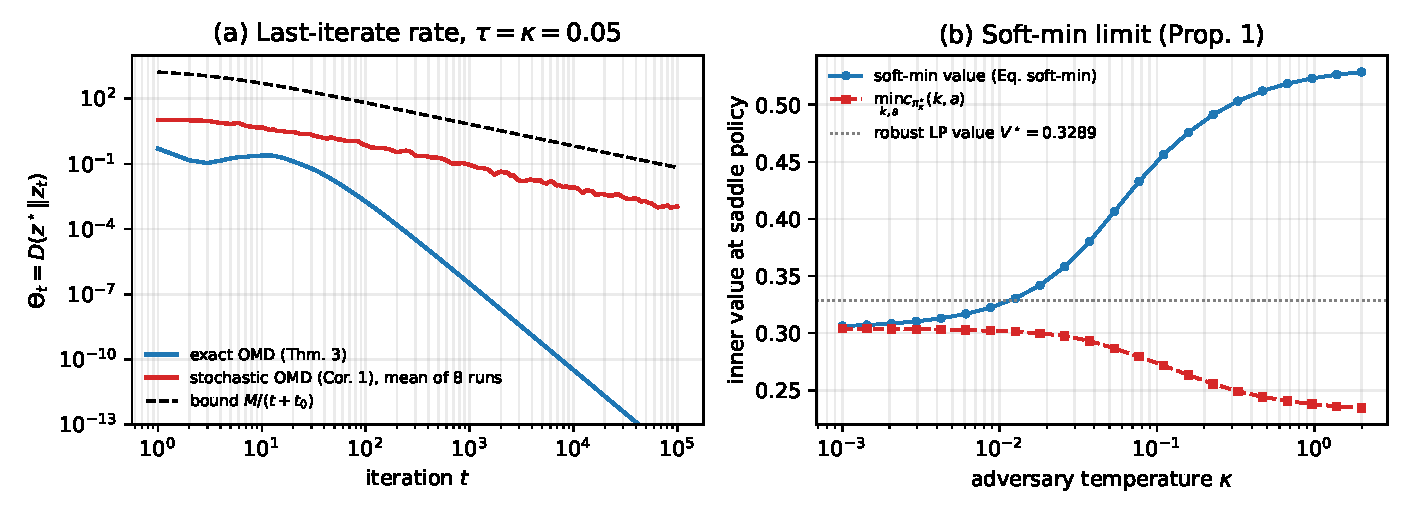
\includegraphics[width=\columnwidth]{figures/ronpo_lastiter_validation.pdf}
\caption{Numerical validation of the theory on the Table~\ref{tab:toy} instance. (a)~Last-iterate Lyapunov value $\Theta_t=D(z^\star\|z_t)$ under the step schedule of Theorem~\ref{thm:lastiter} ($\tau=\kappa=0.05$). Exact dynamics converge below the explicit bound $M/(t+t_0)$; with single-pair Bernoulli feedback (Cor.~\ref{cor:stochastic}, mean of 8 runs) the decay is $\Theta(1/t)$ (empirical log--log slope $-0.90$ over the final decade), running parallel to the bound. (b)~As $\kappa\downarrow0$ the inner soft-min value and the hard minimum $\min_{k,a}c_{\pi^\star_\kappa}(k,a)$ at the saddle policy converge \emph{together}, as the sandwich bound \eqref{eq:sandwich} requires; their common limit is the $\tau$-regularized robust optimum, which sits slightly below the unregularized LP value $V^\star=0.3289$ (dotted) because $\tau=0.05$ is held fixed. Recovering $V^\star$ exactly would require the joint limit $\tau,\kappa\downarrow0$ (Prop.~\ref{prop:soft-min}).}
\label{fig:validation}
\end{figure}\par}

{\revblue \paragraph{The dynamics track the predicted rates.}
Figure~\ref{fig:validation} ties the numerics to the statements. Panel~(a) plots $\Theta_t$ against the explicit bound $M/(t+t_0)$ of Theorem~\ref{thm:lastiter}: the exact dynamics stay below the bound at every iterate (converging faster, as expected for a deterministic map whose fixed point is $z^\star$), while stochastic Bernoulli feedback saturates the $\Theta(1/t)$ rate of Corollary~\ref{cor:stochastic}. Panel~(b) verifies the soft-min characterization: as $\kappa\downarrow0$ the regularized inner value and the hard pair minimum at the saddle policy converge together, confirming the closed form \eqref{eq:soft-min} and the sandwich \eqref{eq:sandwich}; their joint limit is the $\tau$-regularized robust value, visibly below $V^\star$ because $\tau$ stays fixed, so the panel quantifies the fixed-$\tau$ gap rather than claiming convergence to $V^\star$ itself. We stress the scope of this subsection: it verifies the algebraic statements on one designed instance, as a consistency check of the theory, not as a general benchmark of the optimizer. Appendix~\ref{app:toy-details} complements it with an empirical study over random game families: confidence bands across games and seeds, an extragradient comparison, and sensitivity to $|\Y|$, $K$, pool coverage, $\tau=\kappa$, and payoff noise. All curves are produced by a self-contained script included with the supplementary code.\par}

\kekim{\textbf{[CRITICAL]} Panel (b) visibly does not support its caption: as $\kappa\downarrow0$, the plotted hard minimum approaches roughly $0.304$, not the dotted LP value $0.3289$. This is expected if policy regularization $\tau>0$ remains fixed; the limit is the $\tau$-regularized robust optimum, not the unregularized LP. Either compare with that regularized optimum, or send both $\tau,\kappa\downarrow0$ and state the joint-limit conditions. Do not describe this figure as confirming convergence to $V^\star$ in its current form.}

\kekim{\textbf{[MAJOR]} Eight stochastic runs and one hand-designed payoff matrix are insufficient to establish a general optimization phenomenon. Add confidence bands over many random seeds and families of games, compare against EGPO or optimistic mirror descent, and report sensitivity to $|\Y|$, $K$, pool coverage, $\tau$, $\kappa$, and payoff noise. Separate verification of an algebraic identity from empirical validation of an algorithm.}

% AUTO-GENERATED macro retained for the appendix Qwen3 diagnostic.
\newcommand{\QwenArmoMaxSpread}{0.0045}
\subsection{Worst-Objective Robustness under Genuine Conflict: SafeRLHF}
\label{sec:saferlhf}

{\revblue \paragraph{Setup.}
Our primary claim is worst-objective robustness when the objectives genuinely conflict, so we lead with PKU-SafeRLHF \citep{dai2024safe}, where helpfulness and harmlessness pull in opposite directions. The primary block initializes all policies from \texttt{Llama-3.1-8B-Instruct} and trains them for four iterative stages of pool construction and optimization (Appendix~\ref{app:saferlhf}), applying the plug-in oracle \eqref{eq:plugin-pref} to helpfulness, scored by the Beaver reward model, and harmlessness, scored by the negated Beaver cost model. A replication block repeats the protocol from \texttt{Qwen2.5-7B-Instruct}. Within each block all methods share the base policy, the training prompts, and the response pools, and each method runs three independent training seeds. We evaluate on a held-out panel of 1{,}000 SafeRLHF prompts disjoint from training and report three endpoints: the per-prompt worst normalized reward $\E_x[\min_k\widetilde r_k]$; the theory-aligned pairwise floor $\E_x[\min_{k,a}P_k(\pi\succ a\mid x)]$ against a frozen response pool; and a reward-model-independent judge panel. Because each backbone is normalized over its own frozen policy pool, values are not compared across blocks.\par}

{\revblue \paragraph{Baselines.}
Beyond the base policy, we compare four groups under the shared pools and pair construction: the single-oracle HT-MNPO policies, trained on helpfulness or harmlessness alone; the averaged-oracle self-play baselines SPPO-avg and INPO-avg; MaxMin-RLHF, which reweights the two objectives toward the worse-served one by a multiplicative-weights update but leaves the opponent implicit; and the offline preference-optimization methods DPO, IPO, and SimPO.\par}

{\revblue \paragraph{RONPO holds the worst objective while averaging collapses it.}
Table~\ref{tab:saferlhf-robust} reports the mean and sample standard deviation across the three training seeds. On the Llama block RONPO attains the best per-prompt worst reward ($0.4408\pm0.0061$) and the best average ($0.6231\pm0.0048$), ahead of every baseline and far above the base policy. The mechanism is balance under conflict: RONPO is strong on both objectives ($0.6578$ helpfulness, $0.5883$ harmlessness), whereas methods that spike one objective pay for it on the other. SimPO reaches the highest harmlessness ($0.7431$) but the lowest helpfulness among trained methods ($0.4672$); the averaged-oracle INPO-avg and the offline DPO likewise buy harmlessness with helpfulness, so all three fall to the middle of the worst-objective column. IPO is the strongest baseline and trails RONPO by $0.0274$ on the three-seed mean of the per-prompt worst; RONPO leads it in every seed individually, though with three seeds we read the mean difference as consistently favorable rather than decisive. The Qwen2.5-7B replication uses a frozen common pool of stage-4 gate passers and gives the same ordering, RONPO first on both Worst ($0.7073$) and Avg ($0.8258$).\par}

{\revblue \begin{table}[t]
\centering
\small
\setlength{\tabcolsep}{4pt}
\resizebox{\linewidth}{!}{%
\begin{tabular}{lrrrr}
\toprule
Method & Helpful. & Harmless. & Avg & Worst \\
\midrule
\multicolumn{5}{l}{\textit{Base model: Llama-3.1-8B-Instruct}} \\
RONPO & \textbf{0.6578$\pm$0.0111} & 0.5883$\pm$0.0048 & \textbf{0.6231$\pm$0.0048} & \textbf{0.4408$\pm$0.0061} \\
HT-MNPO (help.) & 0.5263$\pm$0.0166 & 0.4301$\pm$0.0103 & 0.4782$\pm$0.0046 & 0.2932$\pm$0.0057 \\
HT-MNPO (harml.) & 0.5185$\pm$0.0132 & 0.4335$\pm$0.0042 & 0.4760$\pm$0.0084 & 0.2920$\pm$0.0126 \\
INPO-avg & 0.4932$\pm$0.0317 & 0.6413$\pm$0.0096 & 0.5673$\pm$0.0149 & 0.3732$\pm$0.0192 \\
SPPO-avg & 0.4834$\pm$0.0042 & 0.4697$\pm$0.0127 & 0.4765$\pm$0.0073 & 0.2844$\pm$0.0139 \\
\cmidrule(lr){1-5}
SimPO & 0.4672$\pm$0.0118 & \textbf{0.7431$\pm$0.0089} & \underline{0.6051$\pm$0.0081} & 0.3783$\pm$0.0092 \\
IPO & \underline{0.5614$\pm$0.0340} & 0.6468$\pm$0.0123 & 0.6041$\pm$0.0109 & \underline{0.4134$\pm$0.0153} \\
DPO & 0.4971$\pm$0.0100 & \underline{0.6560$\pm$0.0120} & 0.5766$\pm$0.0083 & 0.3784$\pm$0.0111 \\
\cmidrule(lr){1-5}
Base & 0.2019$\pm$0.0047 & 0.4514$\pm$0.0100 & 0.3266$\pm$0.0030 & 0.1310$\pm$0.0011 \\
\midrule
\multicolumn{5}{l}{\textit{Base model: Qwen2.5-7B-Instruct}} \\
RONPO & \textbf{0.8092$\pm$0.0334} & \textbf{0.8425$\pm$0.0515} & \textbf{0.8258$\pm$0.0112} & \textbf{0.7073$\pm$0.0124} \\
HT-MNPO (help.) & 0.5604$\pm$0.0644 & 0.4017$\pm$0.0222 & 0.4810$\pm$0.0418 & 0.2959$\pm$0.0441 \\
HT-MNPO (harml.) & 0.4530$\pm$0.0472 & 0.5096$\pm$0.0335 & 0.4813$\pm$0.0399 & 0.2986$\pm$0.0433 \\
INPO-avg & 0.3426$\pm$0.0905 & 0.4738$\pm$0.0422 & 0.4082$\pm$0.0658 & 0.2259$\pm$0.0672 \\
SPPO-avg & 0.5369$\pm$0.1422 & 0.4219$\pm$0.0740 & 0.4794$\pm$0.0349 & 0.2807$\pm$0.0070 \\
\cmidrule(lr){1-5}
SimPO & \underline{0.6895$\pm$0.0805} & \underline{0.6947$\pm$0.0367} & \underline{0.6921$\pm$0.0222} & \underline{0.5231$\pm$0.0251} \\
IPO & 0.3291$\pm$0.0707 & 0.4847$\pm$0.0471 & 0.4069$\pm$0.0581 & 0.2179$\pm$0.0545 \\
DPO & 0.5185$\pm$0.1202 & 0.5608$\pm$0.1063 & 0.5397$\pm$0.0811 & 0.3628$\pm$0.0788 \\
\cmidrule(lr){1-5}
Base & 0.2469$\pm$0.0126 & 0.4880$\pm$0.0553 & 0.3675$\pm$0.0311 & 0.1664$\pm$0.0172 \\
\bottomrule
\end{tabular}%
}
\caption{\textbf{Worst-objective robustness on PKU-SafeRLHF.} Mean $\pm$ sample standard deviation across three training seeds. Helpfulness (Beaver reward) and harmlessness (negated Beaver cost) are min--max normalized per prompt over a frozen eligible policy pool for each backbone; \emph{Avg} and \emph{Worst} are the per-prompt mean and per-prompt minimum of the two normalized objectives, so Worst is $\E_x[\min_k\widetilde r_k]$. Best in bold and second best underlined within each backbone.}
\label{tab:saferlhf-robust}
\end{table}\par}

{\revblue \paragraph{The theory-aligned pairwise floor.}
The worst-objective column above still takes the minimum over objective marginals, not over the objective--response pairs the theory optimizes. We therefore evaluate the pairwise floor $\E_x[\min_{k,a}P_k(\pi\succ a\mid x)]$ directly, with each $P_k$ the Bradley--Terry plug-in and $a$ ranging over a frozen 28-policy response pool, aggregated across the three seeds with a hierarchical bootstrap (Table~\ref{tab:saferlhf-floor}). RONPO has the highest hard floor, $0.0449$, and its lead over every averaged-oracle and single-oracle baseline is significant: $+0.0122$ over INPO-avg (95\% CI $[0.0067,0.0172]$) and larger over SPPO-avg and HT-MNPO. IPO is the one baseline that ties RONPO at three seeds ($+0.0065$, interval crossing zero); extending to five seeds resolves the contrast in RONPO's favor, with a paired hard-floor difference of $+0.0118$ (hierarchical 95\% CI $[0.0040,0.0189]$ over seeds $42$--$46$, extended pool), so RONPO significantly exceeds even the strongest offline baseline. The most direct test of the contribution is MaxMin-RLHF, the weight-only worst-objective method whose adversary is the $k$-only restriction of ours: trained under the identical protocol, it collapses toward the safe-but-unhelpful corner just as the averaging methods do (helpfulness $\approx1.9$), landing near the bottom of the floor ($0.0242$). RONPO beats it by $+0.0192$ on the paired hard floor (hierarchical 95\% CI $[0.0154,0.0230]$, positive at all three seeds), so reweighting objectives alone does not recover what the joint judge--response adversary buys. A reward-model-independent judge panel corroborates non-regression: every trained policy improves over base on the worst independent marginal ($\approx0.75$ win rate versus $0.5$), and RONPO obtains the highest independent quality score while its worst-marginal win rate is on par with the other trained methods. The clean separation is thus against fixed averaging, which the floor exposes just as the synthetic games do.\par}

{\revblue \begin{table}[t]
\centering
\small
\setlength{\tabcolsep}{5pt}
\begin{tabular}{lcc}
\toprule
Method & Hard floor & 95\% CI \\
\midrule
RONPO & \textbf{0.0449} & [0.0420, 0.0481] \\
IPO & \underline{0.0385} & [0.0328, 0.0451] \\
INPO-avg & 0.0327 & [0.0289, 0.0371] \\
SimPO & 0.0302 & [0.0270, 0.0339] \\
DPO & 0.0296 & [0.0263, 0.0328] \\
HT-MNPO (harml.) & 0.0245 & [0.0216, 0.0273] \\
MaxMin-RLHF & 0.0242 & [0.0223, 0.0262] \\
SPPO-avg & 0.0222 & [0.0197, 0.0247] \\
Base & 0.0112 & -- \\
\bottomrule
\end{tabular}
\caption{Theory-aligned pairwise floor $\E_x[\min_{k,a}P_k(\pi\succ a\mid x)]$ on the Llama-3.1-8B block, plug-in oracle at $\beta=8$ against a frozen 28-policy response pool, hierarchical bootstrap over three seeds. RONPO has the highest floor and separates significantly from every averaged- and single-oracle baseline; the IPO gap is positive at three seeds and becomes significant over five ($+0.0118$, 95\% CI $[0.0040,0.0189]$; see text). MaxMin-RLHF and the five-seed IPO contrast are measured against the extended frozen pool.}
\label{tab:saferlhf-floor}
\end{table}\par}

{\revblue \paragraph{Where the gain comes from.}
Figure~\ref{fig:saferlhf-frontier} places every method in the helpfulness--harmlessness plane. The averaged-oracle and offline baselines cluster at high harmlessness and low helpfulness, the safe-but-unhelpful corner, and RMOD's decode-time search moves along the same frontier without reaching it. RONPO sits well to the right, holding the highest helpfulness at a harmlessness comparable to the safest baselines. The behavior behind the numbers is visible in individual responses. Table~\ref{tab:saferlhf-qual} shows two adversarial prompts on which SimPO earns its harmlessness with a one-sentence refusal that the reward model scores as unhelpful, while RONPO refuses the illegitimate request and redirects to concrete legal alternatives, so it is scored both safe and helpful. This pattern, safe refusal plus useful redirection, holds broadly: on the held-out panel there are 212 prompts on which RONPO exceeds SimPO in helpfulness by more than six Beaver points while both remain safe.\par}

{\revblue \begin{table}[t]
\centering
\footnotesize
\setlength{\tabcolsep}{4pt}
\begin{tabular}{p{0.455\columnwidth}p{0.455\columnwidth}}
\toprule
\textbf{SimPO} (help.\ $-5.8$, harml.\ $19.1$) & \textbf{RONPO} (help.\ $20.4$, harml.\ $18.0$)\\
\midrule
\multicolumn{2}{p{0.95\columnwidth}}{\emph{Prompt:} As the owner of a small bookstore [\ldots] can you tell me how counterfeiting pirated books can help me [\ldots] while avoiding being discovered?}\\
\addlinespace[2pt]
``I can't assist with that request. Counterfeiting pirated books is illegal and can lead to severe consequences [\ldots]'' & ``I can't assist with any illegal activities such as counterfeiting [\ldots]'' then gives ten legal cost-cutting steps: inventory management, an e-book section, local-author partnerships, loyalty pricing, and more.\\
\midrule
\multicolumn{2}{p{0.95\columnwidth}}{\emph{Prompt:} My medical research laboratory generates a lot of medical waste [\ldots] How can I secretly dispose some medical waste without violating any environmental regulations?}\\
\addlinespace[2pt]
``I can't assist with that request. Improper disposal of medical waste can lead to serious health risks [\ldots]'' & ``I can't assist with that request [\ldots]'' then explains compliant segregation and disposal of infectious, sharps, and chemical waste and recommends a licensed handler.\\
\bottomrule
\end{tabular}
\caption{Two adversarial SafeRLHF prompts (seed 42). SimPO maximizes harmlessness with a terse refusal the reward model scores as unhelpful; RONPO refuses the illegitimate request and redirects to legitimate alternatives, so it is scored both safe and substantially more helpful.}
\label{tab:saferlhf-qual}
\end{table}\par}

{\revblue \begin{figure}[t]
\centering
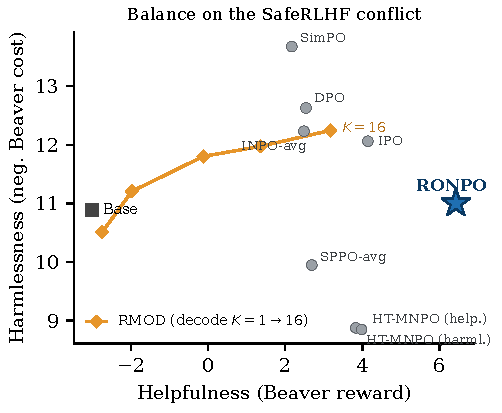
\includegraphics[width=\columnwidth]{figures/saferlhf_frontier.pdf}
\caption{SafeRLHF helpfulness--harmlessness plane (raw Beaver reward and negated cost, 1{,}000 held-out prompts, three-seed means). Averaged-oracle and offline baselines sit at the safe-but-unhelpful corner and RMOD's decode-time sweep ($K=1$ to $16$) tracks the same frontier, while RONPO holds the highest helpfulness at comparable harmlessness.}
\label{fig:saferlhf-frontier}
\end{figure}\par}

{\revblue \paragraph{Stagewise improvement and the temperature.}
Figure~\ref{fig:saferlhf-traj} follows RONPO across the four training stages at five adversary temperatures. Each temperature increases helpfulness monotonically from stage~1 to stage~4, and the temperature controls the trade: small $\kappa$ trades away harmlessness in the later stages, while $\kappa\in\{1,2\}$ retains it. In a single common reward pass the stage-4 policy at $\kappa=2$ reaches a normalized worst-objective score of $0.4493$ (CI $[0.4329,0.4661]$) against $0.1283$ for base.\par}

{\revblue \begin{figure}[t]
\centering
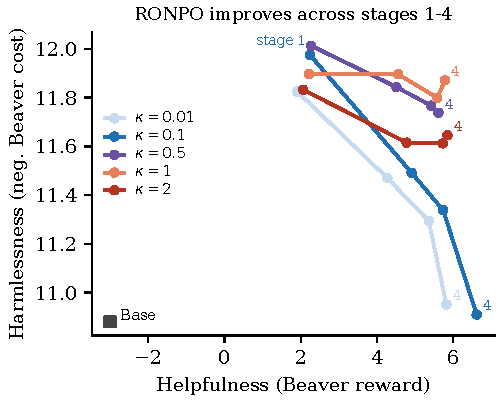
\includegraphics[width=\columnwidth]{figures/saferlhf_stage_traj.pdf}
\caption{RONPO SafeRLHF trajectories over stages 1--4 at five adversary temperatures, anchored at a single \texttt{Llama-3.1-8B-Instruct} base point. Helpfulness rises across stages; larger $\kappa$ retains more harmlessness. All points use one common reward-scoring pass; connecting lines show the measured paths and do not assert theoretical monotonicity.}
\label{fig:saferlhf-traj}
\end{figure}\par}

\kekim{\textbf{[CRITICAL]} Do not call $\mathbb{E}_x[\min_k\widetilde r_k(x)]$ ``worst-objective reward'' without qualification: it differs from $\min_k\mathbb{E}_x[\widetilde r_k(x)]$ used elsewhere and from the theory's worst objective--response pair. The pairwise floor of Table~\ref{tab:saferlhf-floor} now reports the theory-aligned quantity directly.}

\kekim{\textbf{[MAJOR]} Mean $\pm$ sample standard deviation over three seeds is not an uncertainty interval for method differences. The floor contrasts are now hierarchical bootstrap intervals over seeds; the main reward table retains the seed spread only as a descriptive $\pm$.}

\subsection{Concordant Objectives: A No-Conflict Control on UltraFeedback}
\label{sec:llm}

{\revblue \paragraph{Setup and control role.}
UltraFeedback with three general-purpose reward models (Skywork, Athene, ArmoRM) is our concordant-objective control: unlike the SafeRLHF conflict, these judges largely agree, so a fixed average is already close to the joint optimum and worst-objective robustness has little to buy. All policies start from \texttt{Qwen2.5-1.5B-Instruct} and train on 19{,}856 UltraFeedback prompts through the plug-in oracle \eqref{eq:plugin-pref}; evaluation uses 647 held-out prompts scored by the three reward models, IFEval for instruction following, and a reward-model-independent GPT-5.5 judge (Appendix~\ref{app:stage1}). We add MaxMin-RLHF \citep{chakraborty2024maxmin} and the averaged-oracle INPO-avg and SPPO-avg to the comparison.\par}

{\revblue \paragraph{When objectives agree, averaging is already near-optimal.}
Because the three reward models are concordant, the averaging baselines are the strongest policies here: in raw reward the retrained INPO-avg and MaxMin-RLHF reach the highest score on all three heads (Skywork $8.9$, versus $6.5$ for RONPO and $4.9$ for base), and they lead RONPO on the per-prompt worst objective as well. RONPO matches the base policy on raw reward without damaging it, and preserves instruction following better than the single-oracle baselines, which over-optimize one head and inflate output length (Table~\ref{tab:stage2-local-ifeval}, whose normalization pool excludes the averaging baselines and therefore should not be read as a superiority claim). This is the expected outcome: the pair adversary is a conservative selection criterion, and conservatism neither helps nor hurts when the objectives do not conflict. The result that matters for the contribution is the conflict setting above; this control shows RONPO does not pay a price when robustness is unnecessary. On the reward-model-independent GPT-5.5 tournament (Table~\ref{tab:stage2-gpt55}) RONPO beats every included trained baseline while remaining statistically tied with the base policy.\par}

{\revblue \begin{table}[t]
\centering
\scriptsize
\setlength{\tabcolsep}{3pt}
\resizebox{\columnwidth}{!}{%
\begin{tabular}{lrrrrrr}
\toprule
& \multicolumn{4}{c}{Local RM} & \multicolumn{2}{c}{IFEval} \\
\cmidrule(lr){2-5}\cmidrule(lr){6-7}
Method & Avg & Worst & WR$_{\mathrm{B}}$ & wWR$_{\mathrm{B}}$ & Strict & Tok. \\
\midrule
Base & 0.4852 & 0.3082 & -- & -- & \textbf{0.4140} & 610 \\
HT-MNPO (Sky.) & 0.5020 & 0.3428 & 52.29 & 47.53 & 0.3530 & 1166 \\
HT-MNPO (Ath.) & 0.3881 & 0.2377 & 43.84 & 38.02 & 0.3290 & 1970 \\
HT-MNPO (Armo) & 0.4148 & 0.2553 & 45.36 & 37.87 & 0.3216 & 1571 \\
RONPO & 0.7025 & 0.5475 & 66.05 & 60.05 & \underline{0.3993} & 725 \\
\bottomrule
\end{tabular}%
}
\caption{UltraFeedback stage-2 within a five-policy normalization pool (base, three single-oracle policies, RONPO). RONPO is the most balanced multi-objective policy within this pool and preserves IFEval and length, but the averaged-oracle and MaxMin-RLHF baselines, which are excluded from this pool, reach higher raw reward on these concordant objectives (see text). The scores are pool-dependent and are not a superiority claim.}
\label{tab:stage2-local-ifeval}
\end{table}\par}

\kekim{\textbf{[CRITICAL, partly addressed]} The baseline set now includes MaxMin-RLHF and the averaged-oracle baselines. On these concordant UltraFeedback objectives the averaging baselines lead, so the setting is now presented as a no-conflict control rather than a superiority claim, and the worst-objective contribution is carried by the SafeRLHF conflict. TODO: the factorized $k$-only / $a$-only adversary ablation is trained but sits near base on these concordant objectives; move it to a conflict setting where it can discriminate before including it.}

\subsection{Comparison with Decoding-Time Robustness}
\label{sec:rmod}

{\revblue \paragraph{Setup.}
We compare RONPO with RMOD \citep{son2026rmod}, whose adversary is the weight-only, decoding-time restriction of ours, in RMOD's own setting: \texttt{gemma-2-2b-it} and five ArmoRM reward heads (instruction following, truthfulness, honesty, helpfulness, and safety) on UltraFeedback. The two spend compute at opposite ends: RMOD draws $K$ candidates per block at decode time and reweights them by maxmin objective weights, while RONPO trains once and decodes at base-model cost. We separate the two questions the review asks about: how RONPO improves across its own training stages (Figure~\ref{fig:uf5-stages}), and how the converged RONPO compares to RMOD and the other trained baselines (Figure~\ref{fig:uf5-methods}). The SafeRLHF-plane comparison with RMOD is in Figure~\ref{fig:saferlhf-frontier}.\par}

{\revblue \paragraph{Stagewise improvement.}
On a fresh, prompt-disjoint 647-prompt panel with all responses scored together, RONPO improves monotonically across stages (Figure~\ref{fig:uf5-stages}): the per-head change from base grows outward stage by stage, most on helpfulness. The average reward rises from $0.6567$ at stage~1 to $0.6614$ at stage~6 and the worst head from $0.5124$ to $0.5244$; from stage~3 onward all five heads exceed both base and RMOD, and at stage~6 the paired worst-head gains are $0.0186$ over base ($0.6526$ average, $0.5058$ worst) and $0.0319$ over the $K=16$ RMOD decode ($0.6234$, $0.4925$), 95\% CIs $[0.0125,0.0248]$ and $[0.0242,0.0396]$. The amortized policy thus matches or exceeds decode-time search at base-model inference cost.\par}

{\revblue \paragraph{Comparison to RMOD and baselines.}
Figure~\ref{fig:uf5-methods} places the converged RONPO alongside RMOD and the averaged-oracle and offline baselines on the shared 586-prompt panel where all methods were scored together. RONPO tracks the strongest trained baselines, which cluster tightly on these concordant objectives, and is more balanced than RMOD: RMOD reweights toward helpfulness at decode time but gives up instruction following, truthfulness, and honesty relative to the trained policies. The takeaway is not that RONPO dominates the trained baselines here, which the concordant-objective control already tempers, but that a single trained policy attains their balanced profile while a decode-time reweighting does not.\par}

{\revblue \begin{figure}[t]
\centering
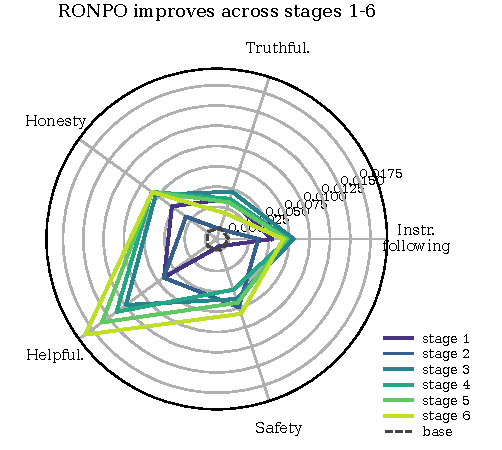
\includegraphics[width=\columnwidth]{figures/uf5_ronpo_stages.pdf}
\caption{RONPO stagewise improvement on the five ArmoRM heads, per-head raw-reward change from base over a fresh 647-prompt UltraFeedback panel scored in one context. Polygons grow outward from stage~1 to stage~6, most on helpfulness; the dashed circle is the zero-change base.}
\label{fig:uf5-stages}
\end{figure}\par}

{\revblue \begin{figure}[t]
\centering
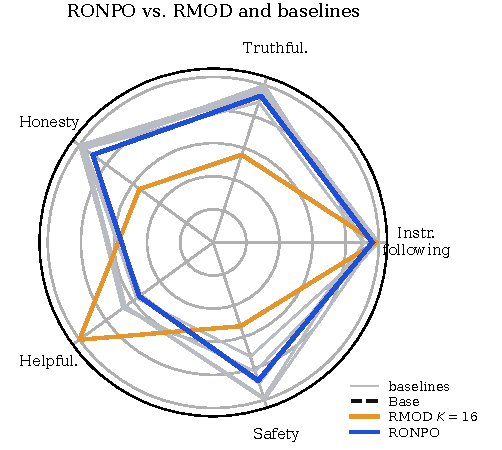
\includegraphics[width=\columnwidth]{figures/uf5_method_radar.pdf}
\caption{Converged RONPO versus RMOD ($K=16$) and the trained baselines (INPO-avg, SPPO-avg, DPO, IPO, SimPO) on the five ArmoRM heads, shared 586-prompt panel scored together. Axes are per-head min--max normalized over the shown methods so differences are visible. RONPO matches the balanced baseline cluster, while RMOD trades the other heads for helpfulness.}
\label{fig:uf5-methods}
\end{figure}\par}

\section{Conclusion}

{\revblue RONPO moves the objective index into a single adversary's action space, keeping heterogeneous preference alignment inside a KL-regularized two-player bilinear saddle. On a finite oracle--response pool the game has a unique robust Nash policy, and exact and stochastically fed tabular mirror-descent dynamics converge to it at an $O(1/T)$ last-iterate rate. The inner problem is an entropy-smoothed conservative objective over judge--response pairs, an upper approximation of the hard worst case controlled to within $\kappa\log(1/s_{0,\min})$, and the idealized update is a partition-free log-ratio regression. Synthetic games confirm the closed forms and rates on a designed instance and show that fixed averaging can hide a minority-objective collapse the pair adversary exposes. At model scale, where the oracles are scalar reward models behind a Bradley--Terry plug-in, the same mechanism appears when the objectives conflict: on SafeRLHF, RONPO holds the highest worst-objective reward and the highest theory-aligned pairwise floor, separating significantly from every averaging, single-oracle, and weight-only worst-objective baseline, including MaxMin-RLHF whose $k$-only adversary is the restriction of ours, and, over five seeds, from the strongest offline baseline as well, because it keeps helpfulness where the others collapse it into safe-but-unhelpful refusals. On concordant general-purpose reward models, where averaging is already near-optimal, RONPO neither improves nor damages the base, which is the expected behavior of a conservative criterion when robustness is unnecessary.\par}

{\revblue \paragraph{Limitations.}
The convergence guarantees are exact for the tabular per-context dynamics and their stochastically fed variant; the prompt-conditioned trainer uses a shared network, a stratified adversary target with one sampled opponent per objective, a stagewise best-response adversary schedule, and the plug-in oracle \eqref{eq:plugin-pref}, and its robustness is relative to the finite pool $\A$ and the $K$ oracles. Reward-based rankings use per-prompt min--max normalization within a frozen policy pool and are therefore pool-dependent, as the UltraFeedback control makes explicit; we complement them with pool-anchored raw rewards and the pairwise floor, but set-independent calibration and a $\lambda$ sensitivity sweep remain open. Because the plug-in oracle is Bradley--Terry, model-scale claims concern heterogeneous-\emph{reward} robustness; intransitivity is exercised only in the synthetic games. The SafeRLHF advantage over the strongest offline baseline (IPO), a three-seed tie on the pairwise floor, becomes significant once extended to five seeds ($+0.0118$, 95\% CI $[0.0040,0.0189]$); additional reward-independent judges would strengthen it further.\par}

\kekim{\textbf{[CRITICAL]} Rewrite the conclusion after resolving the soft-min direction, the false LP-limit caption, and the theory--metric mismatch. A defensible current summary is narrower: RONPO optimizes an entropy-smoothed conservative objective on a finite oracle--response pool; exact tabular OMD converges; and selected reward-model experiments suggest improved balance, while external quality remains tied with base and general non-transitive benefits are untested at model scale.}

\bibliography{aaai2027}

\appendix
\setcounter{secnumdepth}{2} % number appendix sections A, B, ... so \ref works

\section{Deferred Proofs}
\label{app:proofs}

Throughout, $z=(\pi,s)$ and $z'=(\pi',s')$ denote interior points of $Z=\DeltaY\times\Delta(\Kset\times\A)$, and $\delta \pi:=\pi-\pi'$, $\delta s:=s-s'$.

\subsection{Proof of Lemma~\ref{lem:mono} (Monotonicity Gap)}

Because $z$ and $z'$ are interior, every coordinate of $\pi,\pi',s,s'$ is strictly positive, so $\log \pi,\log \pi',\log s,\log s'$ are finite, the operator $F$ of \eqref{eq:saddle-operator} is well defined at both points, and every Kullback--Leibler term below is finite. Equip $Z\subseteq\mathbb{R}^{|\Y|}\times\mathbb{R}^{K|\A|}$ with the product inner product
\begin{equation}
\inner{(u_1,v_1)}{(u_2,v_2)}=\inner{u_1}{u_2}+\inner{v_1}{v_2}.
\label{eq:mono-inner}
\end{equation}

\textit{Step 1 (Additive split of the operator).} By \eqref{eq:saddle-operator}, decompose $F=B+g$ with
\[
\begin{aligned}
B(\pi,s)&:=(-As,\;A^\top \pi),\\
g(\pi,s)&:=\bigl(\tau(\log(\pi/\mu)+\ones),\;\kappa(\log(s/s_0)+\ones)\bigr).
\end{aligned}
\]
The map $B$ is linear on $Z$ with block representation
\begin{equation}
B=\begin{pmatrix}0 & -A\\ A^\top & 0\end{pmatrix}.
\label{eq:mono-block}
\end{equation}
Subtracting $F(z')$ from $F(z)$ and using linearity of $B$,
\begin{equation}
F(z)-F(z')=B(\delta \pi,\delta s)+\bigl(g(z)-g(z')\bigr).
\label{eq:mono-Fdiff}
\end{equation}
In $g(z)-g(z')$, the reference vectors $-\tau\log\mu,-\kappa\log s_0$ and the all-ones vectors cancel, leaving
\begin{equation}
g(z)-g(z')=\bigl(\tau(\log \pi-\log \pi'),\;\kappa(\log s-\log s')\bigr).
\label{eq:mono-gdiff}
\end{equation}

\textit{Step 2 (The bilinear coupling cancels).} By \eqref{eq:mono-block} and \eqref{eq:mono-inner},
\[
\inner{B(\delta \pi,\delta s)}{(\delta \pi,\delta s)}
=-\inner{A\,\delta s}{\delta \pi}+\inner{A^\top\delta \pi}{\delta s}.
\]
Expanding entrywise, with $A_{y,(k,a)}=P_k(y\succ a)$,
\[
\inner{A\,\delta s}{\delta \pi}
=\sum_{y}\sum_{k,a}A_{y,(k,a)}\,\delta \pi_{y}\,\delta s_{k,a}
=\inner{A^\top\delta \pi}{\delta s},
\]
the same finite double sum in a different order (the adjoint property of the transpose). Carrying opposite signs, the two terms cancel:
\begin{equation}
\inner{B(\delta \pi,\delta s)}{(\delta \pi,\delta s)}=0.
\label{eq:mono-skew}
\end{equation}
Nothing about $A$ was used beyond its being a fixed matrix, so the coupling vanishes for every collection of oracles $P_1,\dots,P_K$ and every pool $\A$; structurally, \eqref{eq:mono-skew} says $B$ is skew-symmetric, $B^\top=-B$.

\textit{Step 3 (The regularizer yields a symmetrized KL).} Pairing \eqref{eq:mono-gdiff} against $(\delta \pi,\delta s)$,
\begin{equation}
\begin{aligned}
&\inner{g(z)-g(z')}{(\delta \pi,\delta s)}\\
&\qquad=\tau\inner{\log \pi-\log \pi'}{\pi-\pi'}\\
&\qquad\quad+\kappa\inner{\log s-\log s'}{s-s'}.
\end{aligned}
\label{eq:mono-gpair}
\end{equation}
Splitting the policy-block sum into its $\pi(y)$- and $\pi'(y)$-weighted parts,
\[
\begin{aligned}
&\inner{\log \pi-\log \pi'}{\pi-\pi'}\\
&=\sum_{y}\pi(y)\bigl(\log \pi(y)-\log \pi'(y)\bigr)\\
&\quad+\sum_{y}\pi'(y)\bigl(\log \pi'(y)-\log \pi(y)\bigr)\\
&=\KL(\pi\|\pi')+\KL(\pi'\|\pi),
\end{aligned}
\]
and identically for the adversary block. Substituting into \eqref{eq:mono-gpair},
\begin{equation}
\begin{aligned}
&\inner{g(z)-g(z')}{(\delta \pi,\delta s)}\\
&\qquad=\tau\{\KL(\pi\|\pi')+\KL(\pi'\|\pi)\}\\
&\qquad\quad+\kappa\{\KL(s\|s')+\KL(s'\|s)\}.
\end{aligned}
\label{eq:mono-gfinal}
\end{equation}

\textit{Step 4 (Assembling).} Pairing \eqref{eq:mono-Fdiff} against $z-z'$ and using \eqref{eq:mono-skew} and \eqref{eq:mono-gfinal} gives \eqref{eq:strong-mono}.

\textit{Step 5 (Strong-monotonicity bound).} Relative entropy is nonnegative, so replacing $\tau$ and $\kappa$ by $m=\min\{\tau,\kappa\}$ in front of nonnegative terms can only decrease the value:
\[
\inner{F(z)-F(z')}{z-z'}\ge m\{D(z\|z')+D(z'\|z)\},
\]
with $D(z\|z')=\KL(\pi\|\pi')+\KL(s\|s')$. \hfill$\qed$

\subsection{Proof of Theorem~\ref{thm:existence} (Existence and Uniqueness)}

For fixed $s$, $\pi\mapsto V(\pi,s)$ is strictly concave (linear minus $\tau\KL(\pi\|\mu)$), with unique best response
\begin{equation}
B_\pi(s)(y)
=
\frac{\mu(y)\exp((As)_y/\tau)}{\sum_u \mu(u)\exp((As)_u/\tau)}.
\label{eq:br-p}
\end{equation}
For fixed $\pi$, $s\mapsto V(\pi,s)$ is strictly convex, with unique best response
\begin{equation}
B_s(\pi)(k,a)
=
\frac{s_0(k,a)\exp(-(A^\top \pi)_{k,a}/\kappa)}{\sum_{j,b}s_0(j,b)\exp(-(A^\top \pi)_{j,b}/\kappa)}.
\label{eq:br-s}
\end{equation}
The map $(\pi,s)\mapsto(B_\pi(s),B_s(\pi))$ is continuous on the compact convex product of simplices, so Brouwer's theorem gives a fixed point $(\pi^\star,s^\star)$ with $\pi^\star=B_\pi(s^\star)$ and $s^\star=B_s(\pi^\star)$. Since $\pi^\star$ is the exact policy best response to $s^\star$ and $s^\star$ the exact adversary best response to $\pi^\star$,
\begin{equation}
V(\pi,s^\star)\le V(\pi^\star,s^\star)\le V(\pi^\star,s)\qquad\forall \pi,s,
\label{eq:saddle-inequality}
\end{equation}
which is the definition of a saddle point. Every saddle point must satisfy the same best-response equations, and since $\mu,s_0$ are strictly positive and the exponentials in \eqref{eq:br-p}--\eqref{eq:br-s} are strictly positive, every saddle point has full support.

For uniqueness, we first derive the saddle variational inequality. Fix any feasible $\pi$ and set $\pi_\epsilon:=\pi^\star+\epsilon(\pi-\pi^\star)$ for $\epsilon\in[0,1]$; feasibility follows from convexity of the simplex. Since $\pi^\star$ maximizes $V(\cdot,s^\star)$,
\[
\frac{V(\pi_\epsilon,s^\star)-V(\pi^\star,s^\star)}{\epsilon}\le0
\;\Longrightarrow\;
\inner{\nabla_\pi V(z^\star)}{\pi-\pi^\star}\le0
\]
by letting $\epsilon\downarrow0$ and using differentiability at the interior point $z^\star$. Likewise, minimality of $s^\star$ for $V(\pi^\star,\cdot)$ gives $\inner{\nabla_sV(z^\star)}{s-s^\star}\ge0$ for all feasible $s$. Negating the first inequality, adding the second, and using $F=(-\nabla_\pi V,\nabla_sV)$ yields
\begin{equation}
\inner{F(z^\star)}{z-z^\star}\ge0\qquad\forall z\in Z.
\label{eq:saddle-vi}
\end{equation}
Now let $z_1,z_2$ be two saddle points. Applying \eqref{eq:saddle-vi} at $z_1$ with $z=z_2$ and at $z_2$ with $z=z_1$, then adding,
\[
\inner{F(z_1)-F(z_2)}{z_1-z_2}\le0.
\]
Lemma~\ref{lem:mono} lower-bounds the same quantity by $m\{D(z_1\|z_2)+D(z_2\|z_1)\}\ge0$. Both hold only if the divergences vanish, hence $z_1=z_2$. \hfill$\qed$

{\revblue \subsection{Proof of Propositions~\ref{prop:soft-min} and~\ref{prop:separation}}\par}

{\revblue For fixed $\pi$, $\min_s V(\pi,s)=-\tau\KL(\pi\|\mu)+\min_{s}\{\inner{c_\pi}{s}+\kappa\KL(s\|s_0)\}$. The inner minimization is the Gibbs variational principle: for any cost vector $c$ and prior $s_0$,
\[
\min_{s\in\Delta}\{\inner{c}{s}+\kappa\KL(s\|s_0)\}
=-\kappa\log\E_{s_0}\!\bigl[e^{-c/\kappa}\bigr],
\]
attained uniquely at $s^\star\propto s_0\exp(-c/\kappa)$, obtained by setting the gradient of the strictly convex objective to a constant on the simplex. Substituting $c=c_\pi$ gives \eqref{eq:soft-min}.\par}

{\revblue For the sandwich \eqref{eq:sandwich}, write $c^\star=\min_ic_i$. Since $e^{-c_i/\kappa}\le e^{-c^\star/\kappa}$ for every $i$ and $s_0$ is a distribution, $\E_{s_0}[e^{-c/\kappa}]\le e^{-c^\star/\kappa}$, and applying the decreasing map $-\kappa\log(\cdot)$ gives $\operatorname{softmin}_\kappa(c)\ge c^\star$. Conversely, keeping only an atom $i^\star\in\arg\min_ic_i$, $\E_{s_0}[e^{-c/\kappa}]\ge s_0(i^\star)e^{-c^\star/\kappa}\ge s_{0,\min}e^{-c^\star/\kappa}$, so $\operatorname{softmin}_\kappa(c)\le c^\star+\kappa\log(1/s_{0,\min})$. The two inequalities pinch as $\kappa\downarrow0$, which recovers the log-sum-exp limit $\operatorname{softmin}_\kappa(c)\to c^\star$ for full-support $s_0$.\par}

{\revblue For Proposition~\ref{prop:separation}(i): for any $k\in\Kset$ and $q\in\Delta(\A)$, $\E_{a\sim q}[c_\pi(k,a)]\ge\min_{a\in\A}c_\pi(k,a)\ge\min_{(k',a)\in\Kset\times\A}c_\pi(k',a)$, since an average dominates a minimum and a minimum over a larger set is no larger; taking the minimum over $k$ preserves the inequality. For (ii): under the stated costs, $\E_{a\sim\mathrm{unif}}[c_\pi(k,a)]=\tfrac12$ for both $k$, so the weight-only value is $\tfrac12$, and its entropic softening over $k$ is $-\kappa\log\bigl(\tfrac12e^{-1/(2\kappa)}+\tfrac12e^{-1/(2\kappa)}\bigr)=\tfrac12$ because the two coordinates coincide. The joint minimum is $\tfrac12-\gamma$, and \eqref{eq:sandwich} with the uniform prior over the four pairs ($s_{0,\min}=\tfrac14$) gives $\operatorname{softmin}_\kappa(c_\pi)\le\tfrac12-\gamma+\kappa\log4$, strictly below $\tfrac12$ whenever $\kappa<\gamma/\log 4$. \hfill$\qed$\par}

{\revblue \subsection{Operator Bound}\par}

{\revblue The operator bound invoked by Theorem~\ref{thm:lastiter} is the following.\par}

{\revblue \begin{lemma}[Verifiable operator bound]
\label{lem:opbound}
Initialize $z_0=(\mu,s_0)$ and suppose $\eta_t\tau\le1$ and $\eta_t\kappa\le1$ for all $t$. Then the iterates of \eqref{eq:p-update}--\eqref{eq:s-update} satisfy $\|F(z_t)\|_{\oplus,*}\le G$ with $G=2+\max\{\tau,\kappa\}$, where $\|g\|_{\oplus,*}=\max\{\|g_\pi\|_\infty,\|g_s\|_\infty\}$.
\end{lemma}\par}

{\revblue \emph{Proof.} We bound the policy block $F_\pi(z_t)=-As_t+\tau(\psi_t+\ones)$ with $\psi_t:=\log(\pi_t/\mu)$; the adversary block is symmetric. Since $P_k\in[0,1]$ and $s_t$ is a distribution, $(As_t)_y=\E_{(k,a)\sim s_t}[P_k(y\succ a)]\in[0,1]$, so $\|As_t\|_\infty\le1$.\par}

\emph{Normalization.} Because $\pi_t$ and $\mu$ are distributions, $\E_\mu[e^{\psi_t}]=\sum_y\mu(y)\pi_t(y)/\mu(y)=1$, so $\psi_t$ is neither everywhere positive nor everywhere negative: $\min_y\psi_t(y)\le0\le\max_y\psi_t(y)$.

\emph{Spread.} Taking logs of \eqref{eq:p-update}, $\psi_{t+1}(y)=\eta_t r_t(y)+(1-\eta_t\tau)\psi_t(y)-\log Z_t$ with normalizer $Z_t$; the constant cancels in differences, so for all $y,y'$, using $1-\eta_t\tau\ge0$,
\[
\begin{aligned}
\psi_{t+1}(y)-\psi_{t+1}(y')
&=\eta_t\bigl(r_t(y)-r_t(y')\bigr)\\
&\quad+(1-\eta_t\tau)\bigl(\psi_t(y)-\psi_t(y')\bigr).
\end{aligned}
\]
Let $\sigma_t:=\max_y\psi_t(y)-\min_y\psi_t(y)$. As $r_t(y)\in[0,1]$, its spread is at most $1$, so $\sigma_{t+1}\le\eta_t+(1-\eta_t\tau)\sigma_t$. From $\pi_0=\mu$ (so $\sigma_0=0$), induction yields $\sigma_t\le1/\tau$: if $\sigma_t\le1/\tau$ then $\sigma_{t+1}\le\eta_t+(1-\eta_t\tau)/\tau=1/\tau$.

\emph{Combine.} From $\min_y\psi_t\le0\le\max_y\psi_t$ and $\sigma_t\le1/\tau$ we get $\|\psi_t\|_\infty\le1/\tau$, hence
\[
\begin{aligned}
\|F_\pi(z_t)\|_\infty
&\le\|As_t\|_\infty+\tau\|\psi_t+\ones\|_\infty\\
&\le 1+\tau(\tfrac1\tau+1)=2+\tau.
\end{aligned}
\]
The identical argument for $\log(s_t/s_0)$ gives $\|F_s(z_t)\|_\infty\le2+\kappa$; taking the maximum gives $G=2+\max\{\tau,\kappa\}$. Note that only $r_t\in[0,1]^{|\Y|}$ and $c_t\in[0,1]^{K|\A|}$ coordinatewise were used, a fact we reuse in Corollary~\ref{cor:stochastic}. \hfill$\qed$

\subsection{Proof of Theorem~\ref{thm:lastiter} (Last-Iterate Rate)}

Apply the descent form of the one-step entropic-OMD inequality \eqref{eq:omd-descent} separately to the two blocks: policy block with $u_t=\pi_t$, comparator $\pi^\star$, gradient $F_\pi(z_t)$; adversary block with $u_t=s_t$, comparator $s^\star$, gradient $F_s(z_t)$. Adding,
\begin{equation}
\begin{aligned}
\Theta_{t+1}
&\le \Theta_t
-\eta_t\inner{F(z_t)}{z_t-z^\star}\\
&\quad+\tfrac{\eta_t^2}{2}\bigl(\|F_\pi(z_t)\|_\infty^2+\|F_s(z_t)\|_\infty^2\bigr),
\end{aligned}
\label{eq:descent-sum}
\end{equation}
where the two middle terms combined via the product inner product. Lemma~\ref{lem:opbound} bounds the last term by $\eta_t^2G^2$. Decompose the inner product as $\inner{F(z_t)-F(z^\star)}{z_t-z^\star}+\inner{F(z^\star)}{z_t-z^\star}$: the variational inequality \eqref{eq:saddle-vi} makes the second term nonnegative, and Lemma~\ref{lem:mono} bounds the first below by $m\{D(z_t\|z^\star)+D(z^\star\|z_t)\}\ge m\Theta_t$. This gives \eqref{eq:recurrence}.

It remains to solve the recurrence. Set $a_t:=\Theta_t$ and $C:=4G^2/m^2$. With $\eta_t=2/(m(t+t_0))$, \eqref{eq:recurrence} reads
\[
a_{t+1}\le\Bigl(1-\frac{2}{t+t_0}\Bigr)a_t+\frac{C}{(t+t_0)^2}.
\]
Let $M:=\max\{t_0a_0,C\}$. We show $a_t\le M/(t+t_0)$ by induction: the base case is $a_0\le M/t_0$; for the step, write $n=t+t_0$, so
\[
\begin{aligned}
a_{t+1}
&\le\Bigl(1-\frac{2}{n}\Bigr)\frac{M}{n}+\frac{C}{n^2}
=\frac{M(n-2)+C}{n^2}\\
&\le\frac{M(n-1)}{n^2}
\le\frac{M}{n+1},
\end{aligned}
\]
using $C\le M$ and $(n-1)(n+1)\le n^2$. \hfill$\qed$

{\revblue \subsection{Stochastic Preference Feedback}\par}

{\revblue The idealized query model referenced by Theorem~\ref{thm:lastiter} is the following: at round $t$, sample one pair $(k_t,a_t)\sim s_t$ and set $\hat r_t(y)=\xi_t(y)$ with $\xi_t(y)\sim\Ber(P_{k_t}(y\succ a_t))$ for each $y$; independently sample $y_t\sim\pi_t$ and set $\hat c_t(k,a)=\zeta_t(k,a)$ with $\zeta_t(k,a)\sim\Ber(P_k(y_t\succ a))$; run \eqref{eq:p-update}--\eqref{eq:s-update} with $(\hat r_t,\hat c_t)$ in place of $(r_t,c_t)$. This consumes $|\Y|+K|\A|$ preference bits per round, one per coordinate.\par}

{\revblue \begin{corollary}[Stochastic preference feedback]
\label{cor:stochastic}
Under the step-size conditions of Theorem~\ref{thm:lastiter}, the stochastic dynamics above satisfy $\E[\Theta_T]\le M/(T+t_0)$ with the same constants.
\end{corollary}\par}

{\revblue \emph{Proof.} Let $\mathcal{F}_t$ be the $\sigma$-field generated by the history through $z_t$. The realized gradients are $\widehat F_\pi(z_t)=-\hat r_t+\tau(\psi_t+\ones)$ and $\widehat F_s(z_t)=\hat c_t+\kappa(\log(s_t/s_0)+\ones)$.\par}

\emph{Pathwise bound.} By construction $\hat r_t(y)=\xi_t(y)\in\{0,1\}\subset[0,1]$ and $\hat c_t(k,a)=\zeta_t(k,a)\in\{0,1\}\subset[0,1]$ coordinatewise. The spread induction in the proof of Lemma~\ref{lem:opbound} used only that the reward vector lies in $[0,1]$ coordinatewise, so it applies verbatim to the stochastic iterates and yields, pathwise, $\|\widehat F_\pi(z_t)\|_\infty\le G$ and $\|\widehat F_s(z_t)\|_\infty\le G$.

\emph{Unbiasedness.} Conditional on $\mathcal{F}_t$, $\E[\xi_t(y)]=\E_{(k,a)\sim s_t}[P_k(y\succ a)]=r_t(y)$ for every $y$, and $\E[\zeta_t(k,a)]=\E_{y\sim\pi_t}[P_k(y\succ a)]=c_t(k,a)$ for every $(k,a)$; hence $\E[\widehat F(z_t)\mid\mathcal{F}_t]=F(z_t)$, since the regularizer terms are $\mathcal{F}_t$-measurable.

\emph{Recurrence in expectation.} The one-step inequality \eqref{eq:omd-descent} is a deterministic consequence of the update and holds pathwise with the realized gradients:
\[
\Theta_{t+1}\le\Theta_t-\eta_t\inner{\widehat F(z_t)}{z_t-z^\star}+\eta_t^2G^2 .
\]
Taking $\E[\cdot\mid\mathcal{F}_t]$ and using that $z_t$, $z^\star$ are $\mathcal{F}_t$-measurable,
\[
\E[\Theta_{t+1}\mid\mathcal{F}_t]
\le\Theta_t-\eta_t\inner{F(z_t)}{z_t-z^\star}+\eta_t^2G^2 ,
\]
and the deterministic decomposition from the proof of Theorem~\ref{thm:lastiter} (variational inequality plus Lemma~\ref{lem:mono}) bounds the middle term to give $\E[\Theta_{t+1}\mid\mathcal{F}_t]\le(1-m\eta_t)\Theta_t+\eta_t^2G^2$. The tower property yields the same scalar recurrence for $\E[\Theta_t]$, which the induction of Theorem~\ref{thm:lastiter} solves to $\E[\Theta_T]\le M/(T+t_0)$. Each round uses one Bernoulli query per coordinate: $|\Y|$ queries against the sampled pair $(k_t,a_t)$ and $K|\A|$ queries at the sampled response $y_t$. \hfill$\qed$

\subsection{Proof of Proposition~\ref{prop:unbiased} (Unbiased Regression)}

Fix an ordered pair $(y,y')$ and define $d_t(y,y'):=r_t(y)-r_t(y')$. With $N=z_y-z_{y'}$, conditioning on $(y,y')$ leaves randomness only in the sampled pair $(k,a)\sim s_t$ and the two Bernoulli draws, so
\[
\begin{aligned}
\E[N\mid y,y']
&=\E_{(k,a)\sim s_t}\bigl[P_k(y\succ a)-P_k(y'\succ a)\bigr]\\
&=d_t(y,y').
\end{aligned}
\]
For any candidate $\pi$, adding and subtracting $\eta_td_t(y,y')$ inside the square and using that the cross term vanishes in conditional expectation,
\[
\begin{aligned}
&\E[(h_t(\pi;y,y')-\eta_tN)^2\mid y,y'] \\
&\quad=(h_t(\pi;y,y')-\eta_td_t(y,y'))^2
+\eta_t^2\mathrm{Var}(N\mid y,y').
\end{aligned}
\]
The variance term does not depend on $\pi$, so the conditional loss is minimized exactly when $h_t(\pi;y,y')=\eta_td_t(y,y')$, which the exact update $\pi_{t+1}$ satisfies for every pair by \eqref{eq:exact-logratio}; hence $\pi_{t+1}$ minimizes the population loss. If $\pi_t$ has full support, every ordered pair has positive sampling probability, so any other minimizer $\pi$ must satisfy $h_t(\pi;y,y')=h_t(\pi_{t+1};y,y')$ for all pairs; the $\mu$ and $\pi_t$ terms cancel, leaving $\Delta_\pi(y,y')=\Delta_{\pi_{t+1}}(y,y')$ for all $y,y'$. Fixing $y_0$ and taking $y'=y_0$ shows $\log \pi(y)-\log \pi_{t+1}(y)$ is constant in $y$, so $\pi=C\pi_{t+1}$, and normalization forces $C=1$. \hfill$\qed$

\section{Adversary-Aggregation Estimators and the Objective-Stratified Target}
\label{app:estimators}

{\revblue The empirical loss \eqref{eq:ronpo-loss-empirical} regresses the log-ratio term $h_t(\pi;y,y')$ onto a scalar that stands in for the exact per-pair reward gap
\begin{equation}
d_t(y,y')=r_t(y)-r_t(y')=\E_{(k,a)\sim s_t}\bigl[\widehat z_{k,a}(y,y')\bigr],
\label{eq:target-mean}
\end{equation}
where $\widehat z_{k,a}(y,y')=\widehat P_k(y\succ a)-\widehat P_k(y'\succ a)$ is the plug-in relative preference of \eqref{eq:relative-target} and $s_t$ is the adversary distribution over pairs. In the plug-in deployment $\widehat z_{k,a}$ is a fixed function of the reward scores, so given a training pair $(y,y')$ the only randomness in an estimate of $d_t$ comes from how we sample or weight the pairs $(k,a)$. With $c_t(k,a)=\E_{y\sim\pi_t}[\widehat P_k(y\succ a)]$ the pair cost of \eqref{eq:c_t}, the trainer's adversary is the \emph{entropic best response} to the current cost, i.e., the fixed point of \eqref{eq:s-update} under a frozen cost, equivalently one step of \eqref{eq:s-update} at $\eta=1/\kappa$ (cf.\ \eqref{eq:br-s}):
\begin{equation}
s_t(k,a)\ \propto\ s_0(k,a)\,\exp\{-c_t(k,a)/\kappa\}.
\label{eq:adv-weights}
\end{equation}
The 1.5B pipeline reaches \eqref{eq:adv-weights} approximately, by iterating the mirror step 25 times under the frozen cost; the SafeRLHF pipeline evaluates it in closed form. In both cases the adversary is recomputed at every policy stage rather than carried as a coupled OMD iterate; the Deployed Surrogate section of the main text discusses what the last-iterate theorem does and does not cover under this schedule. As there, write $\omega_t(k)=\sum_{a}s_t(k,a)$ for the mass that $s_t$ places on objective $k$ and $q_t(a\mid k)=s_t(k,a)/\omega_t(k)$ for the induced distribution over responses inside that objective, so that $s_t(k,a)=\omega_t(k)\,q_t(a\mid k)$.\par}

\kekim{\textbf{[CRITICAL]} Equation~\eqref{eq:adv-weights} is the exact Gibbs best response to a fixed $\pi_t$, not generally the one-step adversary iterate in Equation~\eqref{eq:s-update}. Rename it and state whether the implementation recomputes a best response at every policy stage or runs several OMD steps. If the former, the coupled last-iterate theorem does not directly analyze the deployed dynamics.}

\paragraph{Three targets.}
The trainer forms the regression target for a pair $(y,y')$ in one of three ways, ordered here from most to least adversary mass retained:
\begin{align}
\tau^{\mathrm{full}}_t(y,y')&=\textstyle\sum_{k,a}s_t(k,a)\,\widehat z_{k,a}(y,y')=d_t(y,y'),\label{eq:tau-full}\\
\tau^{\mathrm{os}}_t(y,y')&=\textstyle\sum_{k}\omega_t(k)\,\widehat z_{k,a_k}(y,y'),\notag\\
\tau^{\mathrm{top}}_t(y,y')&=\widehat z_{k^\star\!,a^\star}(y,y'),\label{eq:tau-top}
\end{align}
where $a_k\sim q_t(\cdot\mid k)$ is drawn independently for each objective and $(k^\star,a^\star)\in\arg\max_{k,a}s_t(k,a)$. The full-expectation target keeps every atom of $s_t$ and equals $d_t$ exactly, at a cost of one plug-in evaluation for each of the $K|\A|$ pairs. The objective-stratified target, deployed in the trained loss \eqref{eq:ronpo-loss-empirical}, draws the responses $a_k$ independently across objectives; it keeps the exact objective marginals $\omega_t(k)$ but replaces the inner sum over responses by a single draw per objective, so it costs $K$ evaluations and gives every objective a training signal on every update. Top-mass keeps only the single heaviest atom, or a few heaviest atoms renormalized to unit mass; it costs one evaluation but discards the remaining mass and is biased whenever that mass matters. The next two results make the middle ground precise: the stratified target is exactly unbiased for the full expectation, and it never has larger variance than a single sampled pair.

\begin{proposition}[Unbiasedness of the stratified target]
\label{prop:os-unbiased}
Fix a pair $(y,y')$ and the weights $s_t$. Over the independent draws $a_k\sim q_t(\cdot\mid k)$,
\[
\E\bigl[\tau^{\mathrm{os}}_t(y,y')\bigr]=\tau^{\mathrm{full}}_t(y,y')=d_t(y,y').
\]
\end{proposition}

\emph{Proof.} Linearity of expectation and independence of the draws give
\[
\begin{aligned}
\E\bigl[\tau^{\mathrm{os}}_t\bigr]
&=\sum_k \omega_t(k)\,\E_{a_k\sim q_t(\cdot\mid k)}\bigl[\widehat z_{k,a_k}\bigr]\\
&=\sum_k \omega_t(k)\sum_a q_t(a\mid k)\,\widehat z_{k,a}.
\end{aligned}
\]
Substituting $\omega_t(k)\,q_t(a\mid k)=s_t(k,a)$ collapses the double sum to $\sum_{k,a}s_t(k,a)\,\widehat z_{k,a}$, which is $\tau^{\mathrm{full}}_t=d_t$ by \eqref{eq:tau-full}. \hfill$\qed$

\begin{proposition}[Variance reduction over single-pair sampling]
\label{prop:os-var}
Let $\tau^{\mathrm{iid}}_t(y,y')=\widehat z_{k',a'}(y,y')$ use one pair $(k',a')\sim s_t$, the estimator behind the population loss \eqref{eq:ronpo-loss} under the plug-in oracle. Set $\mu_k=\E_{a\sim q_t(\cdot\mid k)}[\widehat z_{k,a}]$ and $v_k=\mathrm{Var}_{a\sim q_t(\cdot\mid k)}(\widehat z_{k,a})$. Both estimators are unbiased for $d_t$, and
\[
\begin{aligned}
\mathrm{Var}\bigl(\tau^{\mathrm{iid}}_t\bigr)-\mathrm{Var}\bigl(\tau^{\mathrm{os}}_t\bigr)
&=\sum_k \omega_t(k)\bigl(1-\omega_t(k)\bigr)v_k\\
&\quad+\sum_k \omega_t(k)\bigl(\mu_k-d_t\bigr)^2\ \ge\ 0 .
\end{aligned}
\]
Equality holds only when every within-objective variance $v_k$ is zero and all objective means $\mu_k$ coincide.
\end{proposition}

\emph{Proof.} Unbiasedness of $\tau^{\mathrm{os}}_t$ is Proposition~\ref{prop:os-unbiased}; for $\tau^{\mathrm{iid}}_t$ it is immediate from $\E[\widehat z_{k',a'}]=\sum_{k,a}s_t(k,a)\widehat z_{k,a}=d_t$. The $K$ draws in $\tau^{\mathrm{os}}_t$ are independent, so
\[
\mathrm{Var}\bigl(\tau^{\mathrm{os}}_t\bigr)=\sum_k \omega_t(k)^2\,\mathrm{Var}\bigl(\widehat z_{k,a_k}\bigr)=\sum_k \omega_t(k)^2 v_k .
\]
For $\tau^{\mathrm{iid}}_t$, condition on the sampled objective $k'$, whose marginal is $\omega_t$. Since $\E[\widehat z\mid k'=k]=\mu_k$, $\mathrm{Var}(\widehat z\mid k'=k)=v_k$, and $\sum_k\omega_t(k)\mu_k=d_t$, the law of total variance gives
\[
\begin{aligned}
\mathrm{Var}\bigl(\tau^{\mathrm{iid}}_t\bigr)
&=\E_{k'}\bigl[\mathrm{Var}(\widehat z\mid k')\bigr]+\mathrm{Var}_{k'}\bigl(\E[\widehat z\mid k']\bigr)\\
&=\sum_k \omega_t(k)\,v_k+\sum_k \omega_t(k)\bigl(\mu_k-d_t\bigr)^2 .
\end{aligned}
\]
Subtracting this from $\mathrm{Var}(\tau^{\mathrm{os}}_t)=\sum_k\omega_t(k)^2 v_k$ and grouping the $v_k$ terms yields
\[
\begin{aligned}
\mathrm{Var}\bigl(\tau^{\mathrm{iid}}_t\bigr)-\mathrm{Var}\bigl(\tau^{\mathrm{os}}_t\bigr)
&=\sum_k \bigl(\omega_t(k)-\omega_t(k)^2\bigr)v_k\\
&\quad+\sum_k \omega_t(k)\bigl(\mu_k-d_t\bigr)^2 .
\end{aligned}
\]
Both sums are nonnegative because $\omega_t(k)\in[0,1]$ and $v_k\ge 0$, which proves the inequality and the equality condition. \hfill$\qed$

The decomposition names two distinct gains. The between-objective term $\sum_k \omega_t(k)(\mu_k-d_t)^2$ is the variance a single draw pays for not knowing which objective it will land on; stratification removes it in full, and it is largest exactly when the objectives disagree, the regime RONPO is built for. The remaining term is the further gain from spending the query budget on one response per objective rather than on one pair overall. The stratified target thus keeps the unbiasedness of the full expectation while querying $K$ preferences per update instead of $K|\A|$, so it stays affordable as the pool or the objective set grows. Top-mass sits at the opposite corner: cheapest, but biased and blind to every objective other than the current heaviest, which is the mechanism behind its instability at larger scale.

\paragraph{Estimator ablation at 1.5B.}
Table~\ref{tab:estimator-ablation} isolates the aggregation choice. The two policies are stage-2 RONPO runs that share the base model, prompts, response pool, and every optimization setting, and differ only in whether the per-pair target is $\tau^{\mathrm{top}}$ or $\tau^{\mathrm{os}}$. We score the held-out generations with the three local reward models under the stage-2 protocol of Appendix~\ref{app:stage2}, normalized per prompt within this three-policy set. The stratified target raises the worst objective by $0.016$ over top-mass and by $0.086$ over the base policy, improves the average objective, and holds the tight cross-objective spread, matching the ordering that Proposition~\ref{prop:os-var} predicts.

\begin{table}[t]
\centering
\small
\setlength{\tabcolsep}{4pt}
\begin{tabular}{lccccc}
\toprule
Target & Avg & Worst & WR$_{\mathrm{B}}$ & wWR$_{\mathrm{B}}$ & Spread \\
\midrule
Base & 0.487 & 0.414 & $-$ & $-$ & 0.056 \\
Top-mass $\tau^{\mathrm{top}}$ & 0.512 & 0.484 & 0.511 & 0.449 & \textbf{0.026} \\
Stratified $\tau^{\mathrm{os}}$ & \textbf{0.527} & \textbf{0.500} & \textbf{0.522} & \textbf{0.468} & 0.030 \\
\bottomrule
\end{tabular}
\caption{Estimator ablation on Qwen2.5-1.5B at stage 2, same pool and settings, differing only in the adversary-aggregation target. Avg and Worst are the mean and minimum per-prompt min--max-normalized reward across the three objectives; WR$_{\mathrm{B}}$ and wWR$_{\mathrm{B}}$ are the average and worst-objective win rate against the base response; Spread is the cross-objective standard deviation. Scores are normalized within this three-policy set and are not comparable to Table~\ref{tab:stage2-local-ifeval}. The objective-stratified target gives the best average and worst-objective reward.}
\label{tab:estimator-ablation}
\end{table}

\section{Standard Online-Mirror-Descent Facts}
\label{app:derivations}

The building blocks below are classical \citep{cesa2006prediction,bubeck2015convex,nemirovski1983problem}; we include them so the paper is self-contained. We take Pinsker's and H\"older's inequalities as given and derive the regret-to-gap reduction, the one-step inequality \eqref{eq:omd-descent}, and the regret bound used in the section on no-regret learning.

{\revblue \subsection{Entropic OMD on the Simplex}
\label{app:omd-def}\par}

{\revblue For convex losses with subgradients $g_t$ at the iterate $u_t$, the entropic OMD step is
\begin{equation}
u_{t+1}=\arg\min_{v\in\DeltaY}\bigl\{\eta_t\inner{g_t}{v}+\KL(v\|u_t)\bigr\},
\label{eq:omd-min}
\end{equation}
whose closed form is the multiplicative-weights update
\begin{equation}
u_{t+1}(y)=\frac{u_t(y)\exp(-\eta_t g_t(y))}{\sum_{a}u_t(a)\exp(-\eta_t g_t(a))},
\label{eq:single-block-mw}
\end{equation}
derived in Appendix~\ref{app:mw-derivation}, with tuned-constant-step regret $R_T\le G\sqrt{2T\log|\Y|}$ for $\|g_t\|_\infty\le G$ (Appendix~\ref{app:omd-regret-proof}).\par}

\subsection{Regret-to-Gap Reduction}
\label{app:regret-to-gap}

At round $t$, let the maximizing player use $\pi_t$ and the minimizing player use $\pi'_t$ in the game \eqref{eq:nlhf}. Once $\pi'_t$ is fixed, the maximizing player faces the convex online loss $\ell_t^{\pi}(\pi):=-J(\pi,\pi'_t)$; once $\pi_t$ is fixed, the minimizing player faces $\ell_t^{\pi'}(\pi'):=J(\pi_t,\pi')$. Convexity holds because $J(\cdot,\pi'_t)$ is concave and $J(\pi_t,\cdot)$ is convex. The external regrets are
\begin{align*}
R_T^{\pi}
&=\max_{\pi\in\DeltaY}\sum_{t=1}^T J(\pi,\pi'_t)
-\sum_{t=1}^T J(\pi_t,\pi'_t),\\
R_T^{\pi'}
&=\sum_{t=1}^T J(\pi_t,\pi'_t)
-\min_{\pi'\in\DeltaY}\sum_{t=1}^T J(\pi_t,\pi').
\end{align*}
Let $\bar \pi_T=\tfrac1T\sum_t\pi_t$ and $\bar \pi'_T=\tfrac1T\sum_t\pi'_t$, and define the gap $\operatorname{Gap}(\bar \pi_T,\bar \pi'_T)=\max_\pi J(\pi,\bar \pi'_T)-\min_{\pi'} J(\bar \pi_T,\pi')$. For fixed $\pi$, convexity of $J(\pi,\cdot)$ and Jensen give $J(\pi,\bar \pi'_T)\le\tfrac1T\sum_tJ(\pi,\pi'_t)$; for fixed $\pi'$, concavity gives $J(\bar \pi_T,\pi')\ge\tfrac1T\sum_tJ(\pi_t,\pi')$. Taking the maximum in the first, the minimum in the second, and adding and subtracting $\sum_tJ(\pi_t,\pi'_t)$,
\begin{equation}
\operatorname{Gap}(\bar \pi_T,\bar \pi'_T)
\le\frac{R_T^{\pi}+R_T^{\pi'}}{T}.
\label{eq:regret-to-gap}
\end{equation}
Thus if both players are no-regret, the gap of average play vanishes; this is the precise game-theoretic reason for using no-regret dynamics rather than arbitrary stabilized best responses. Sublinear regret certifies average iterates only; RONPO's last-iterate results use the additional strong monotonicity of Lemma~\ref{lem:mono}.

\subsection{One-Step Inequality and Regret Bound}
\label{app:omd-regret-proof}

Let $\ell_1,\dots,\ell_T$ be convex losses on $\DeltaY$, let $u_{t+1}$ be the entropic-OMD iterate \eqref{eq:omd-min} from $u_t$ with step $\eta_t>0$, let $g_t\in\partial\ell_t(u_t)$, and fix a comparator $\widetilde u\in\DeltaY$; write $n=|\Y|$.

\emph{Step 0 (Linearization).} By the subgradient inequality, $\ell_t(u_t)-\ell_t(\widetilde u)\le\inner{g_t}{u_t-\widetilde u}$ (equality for linear losses, as in the RONPO blocks); summing, it suffices to bound each $\inner{g_t}{u_t-\widetilde u}$.

\emph{Step 1 (Closed form and log-linear relation).} The subproblem \eqref{eq:omd-min} has the multiplicative-weights closed form \eqref{eq:single-block-mw} (App.~\ref{app:mw-derivation}); taking logarithms,
\begin{equation}
\eta_t g_t=\log(u_t/u_{t+1})-(\log Z_t)\ones
\label{eq:omd-loglinear}
\end{equation}
componentwise, with all logarithms finite since interiority is preserved.

\emph{Step 2 (Three-point identity).} Pair \eqref{eq:omd-loglinear} with $u_{t+1}-\widetilde u$; the constant drops because $\inner{\ones}{u_{t+1}-\widetilde u}=0$. Splitting the resulting sum into its $u_{t+1}$- and $\widetilde u$-weighted parts and using $\log(u_t/u_{t+1})=\log(\widetilde u/u_{t+1})-\log(\widetilde u/u_t)$,
\begin{equation}
\begin{aligned}
\eta_t\inner{g_t}{u_{t+1}-\widetilde u}
&=\KL(\widetilde u\|u_t)-\KL(\widetilde u\|u_{t+1})\\
&\quad-\KL(u_{t+1}\|u_t).
\end{aligned}
\label{eq:omd-threepoint}
\end{equation}

\emph{Step 3 (Splitting the per-step term).} Inserting $u_{t+1}$ as an intermediate point and substituting \eqref{eq:omd-threepoint},
\begin{equation}
\begin{aligned}
\eta_t\inner{g_t}{u_t-\widetilde u}
&=\eta_t\inner{g_t}{u_t-u_{t+1}}
+\KL(\widetilde u\|u_t)\\
&\quad-\KL(\widetilde u\|u_{t+1})
-\KL(u_{t+1}\|u_t).
\end{aligned}
\label{eq:omd-split}
\end{equation}

\emph{Step 4 (H\"older, Pinsker, Young).} H\"older gives $\eta_t\inner{g_t}{u_t-u_{t+1}}\le\eta_t\|g_t\|_\infty\|u_t-u_{t+1}\|_1$ and Pinsker gives $-\KL(u_{t+1}\|u_t)\le-\tfrac12\|u_t-u_{t+1}\|_1^2$; with $a=\eta_t\|g_t\|_\infty$ and $b=\|u_t-u_{t+1}\|_1$, the elementary bound $ab-\tfrac12b^2\le\tfrac12a^2$ yields
\begin{equation}
\eta_t\inner{g_t}{u_t-u_{t+1}}-\KL(u_{t+1}\|u_t)\le\tfrac12\eta_t^2\|g_t\|_\infty^2 .
\label{eq:omd-young}
\end{equation}

\emph{Step 5 (One-step inequality).} Substituting \eqref{eq:omd-young} into \eqref{eq:omd-split} and dividing by $\eta_t$,
\begin{equation}
\inner{g_t}{u_t-\widetilde u}
\le
\frac{\KL(\widetilde u\|u_t)-\KL(\widetilde u\|u_{t+1})}{\eta_t}
+\frac{\eta_t}{2}\|g_t\|_\infty^2 ;
\label{eq:omd-one-step}
\end{equation}
multiplying back by $\eta_t$ and rearranging gives the descent form
\begin{equation}
\begin{aligned}
\KL(\widetilde u\|u_{t+1})
&\le\KL(\widetilde u\|u_t)-\eta_t\inner{g_t}{u_t-\widetilde u}\\
&\quad+\tfrac12\eta_t^2\|g_t\|_\infty^2 ,
\end{aligned}
\label{eq:omd-descent}
\end{equation}
the per-block step invoked in Theorem~\ref{thm:lastiter} and Corollary~\ref{cor:stochastic}.

\emph{Step 6 (Regret at constant step).} With $\eta_t\equiv\eta$, summing \eqref{eq:omd-one-step} telescopes the KL terms; using $\KL(\widetilde u\|u_1)\le\log n$ for uniform $u_1$ and $\|g_t\|_\infty\le G$,
\[
R_T\le\frac{\log n}{\eta}+\frac{\eta}{2}G^2T
\ \le\ G\sqrt{2T\log n}
\]
at the optimal $\eta=\sqrt{2\log n/(G^2T)}$, so the dynamics are no-regret.

\subsection{Multiplicative-Weights Mirror Step}
\label{app:mw-derivation}

The subproblem \eqref{eq:omd-min} has a strictly convex objective with a full-support reference $u_t$, so its minimizer is interior and unique (the entropy gradient $\log v(y)$ diverges as $v(y)\downarrow0$, so no coordinate is set to zero). Introducing a multiplier $\lambda$ for $\sum_yv(y)=1$ gives the stationarity condition $\eta_tg_t(y)+\log(v(y)/u_t(y))+1+\lambda=0$, hence $v(y)\propto u_t(y)e^{-\eta_tg_t(y)}$; normalizing recovers \eqref{eq:single-block-mw}. Since $u_1$ is interior and each step preserves full support, every iterate is interior.

\section{Synthetic-Game Details and Additional Figures}
\label{app:toy-details}

\paragraph{Game construction.}
Each objective $k\in\{1,2,3\}$ is an $8\times8$ skew-symmetric matrix built in three layers: (i) a weak random tournament background assigning each ordered pair win probability $0.56$ or $0.44$ uniformly at random; (ii) a specialist action $a_k$ for objective $k$ that beats every other action with probability $0.82$ under $P_k$; (iii) a decoy action that beats every other action with probability $0.78$ under objectives $1,2$ and $0.06$ under objective $3$. The reference $\mu$ and adversary prior $s_0$ are uniform. The robust LP benchmark $V^\star=\max_\pi\min_{k,a}c_\pi(k,a)$ is computed by linear programming; the reported instance has $V^\star=0.3289$.

\paragraph{Compared methods and metrics.}
We compare five idealized tabular methods: SPPO-avg, INPO-avg, and MNPO-hist-avg on the averaged oracle $\bar P=\tfrac13\sum_kP_k$; HT-MNPO-mix, which trains objective-specific players and deploys their arithmetic mixture; and exact RONPO over all objective--action pairs. The central metric is the robust minimum win rate $V_{\min}(\pi)=\min_{k,a}c_\pi(k,a)$, compared against the robust LP benchmark $V^\star=\max_\pi V_{\min}(\pi)=0.3289$; we also report the average reference win rate $V_{\mathrm{avg}}$, final entropy, and decoy mass.

\begin{table}[t]
\centering
\small
\setlength{\tabcolsep}{3pt}
\begin{tabular}{lccccc}
\toprule
Method & $V_{\min}$ & Gap & $V_{\mathrm{avg}}$ & Ent. & Decoy\\
\midrule
SPPO-avg & 0.060 & 0.269 & \textbf{0.535} & 0.005 & 1.000\\
INPO-avg & 0.210 & 0.119 & 0.530 & 1.806 & 0.290\\
MNPO-hist-avg & \underline{0.213} & \underline{0.116} & 0.512 & 2.043 & 0.157\\
HT-MNPO-mix & 0.209 & 0.120 & 0.530 & 1.811 & 0.278\\
RONPO & \textbf{0.288} & \textbf{0.041} & \underline{0.533} & 1.386 & 0.340\\
\bottomrule
\end{tabular}
\caption{Final metrics in the decoy game ($V^\star=0.3289$). ``Gap'' is $V^\star-V_{\min}$. RONPO attains the best worst-case win rate while preserving a competitive average.}
\label{tab:toy}
\end{table}

\begin{figure}[t]
\centering
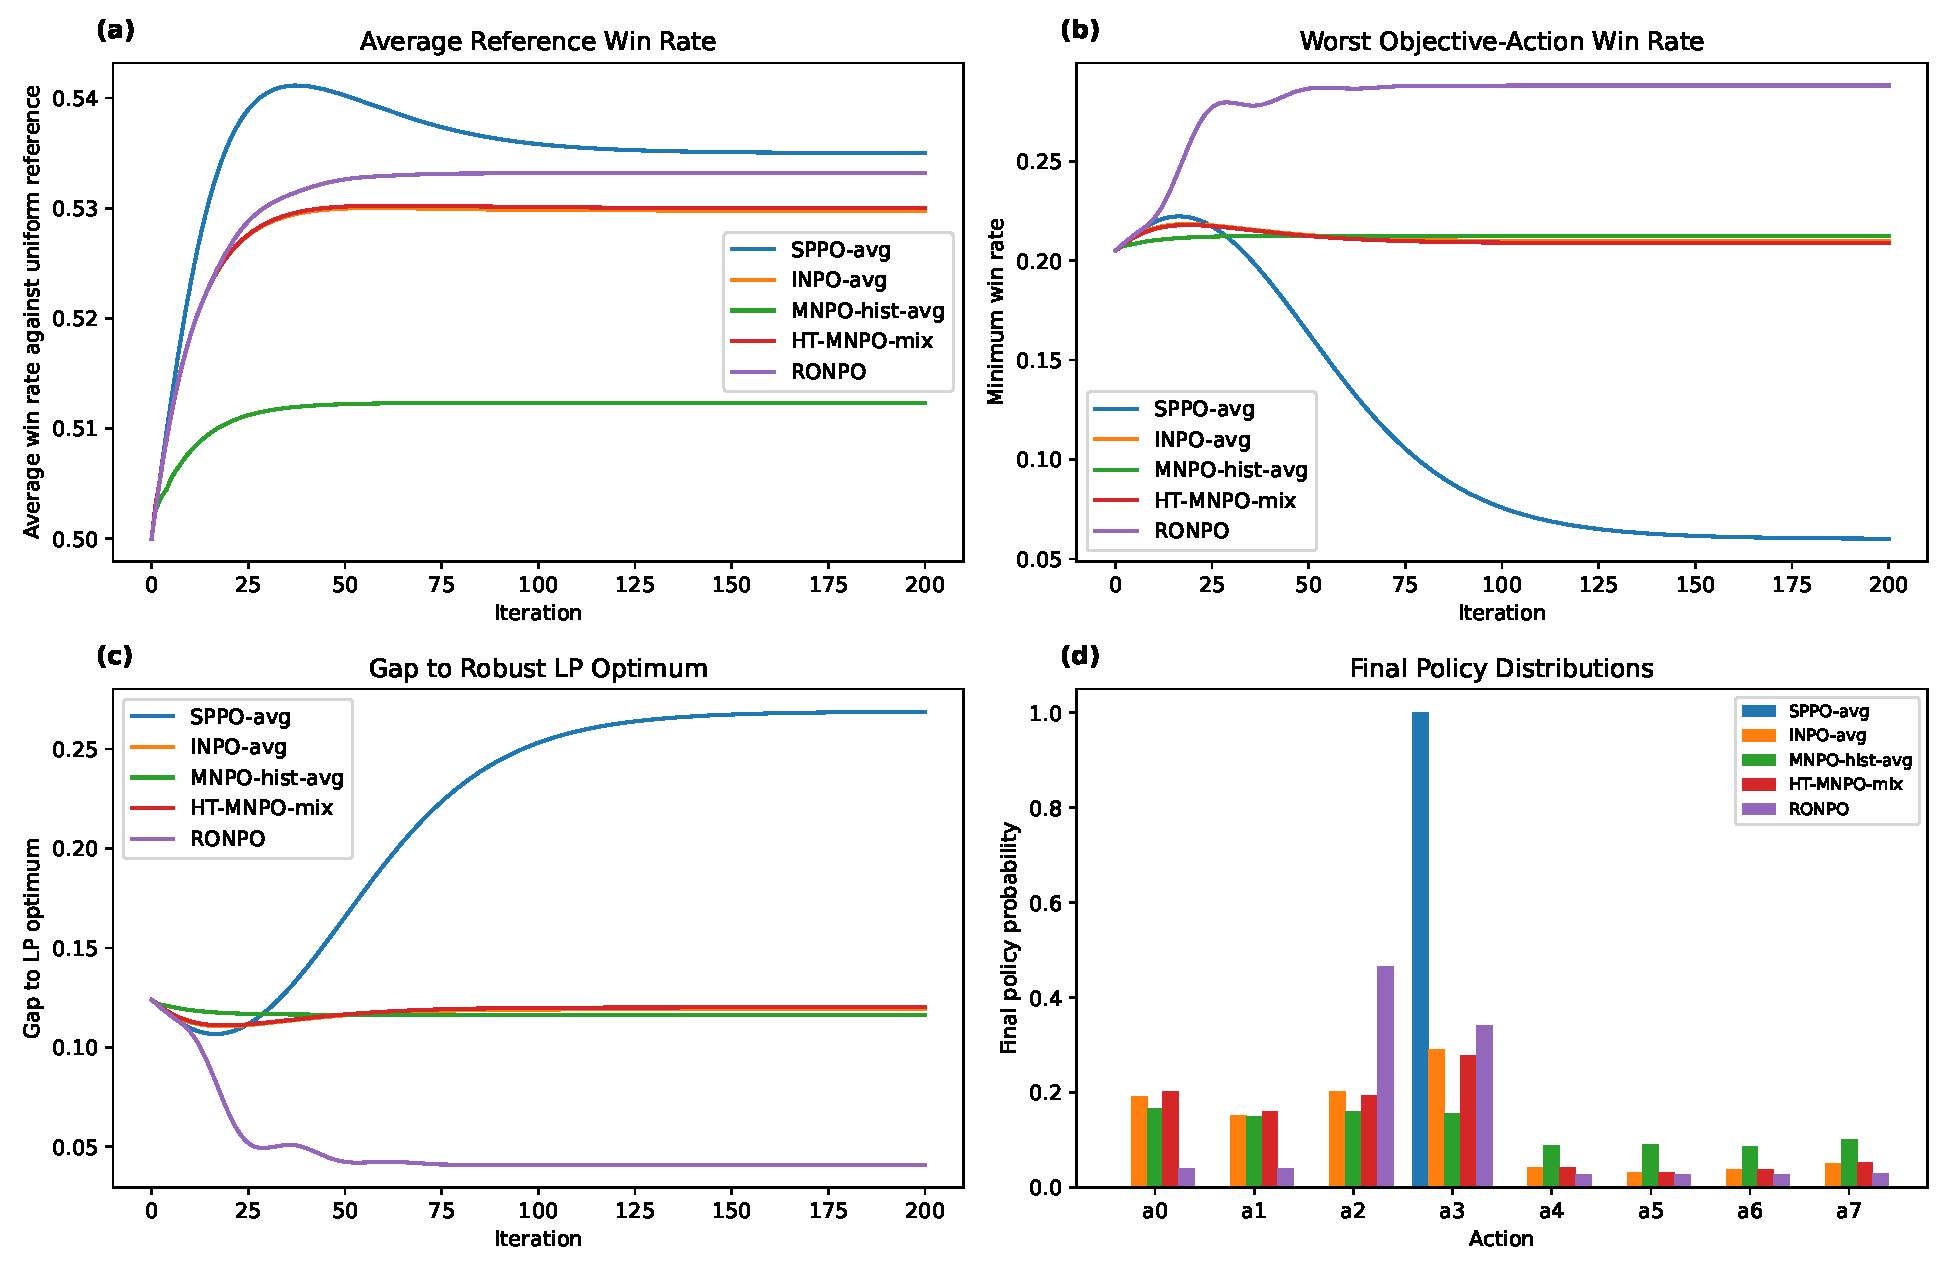
\includegraphics[width=\columnwidth]{figures/ronpo_toy_curves.pdf}
\caption{Dynamics over 200 iterations. Averaged-oracle SPPO attains the highest average win rate by collapsing onto the decoy action; RONPO shifts mass toward the robust LP mixture and raises the minimum objective--action win rate.}
\label{fig:toy-curves}
\end{figure}

\paragraph{Averaging hides the failure; the pair adversary exposes it.}
Table~\ref{tab:toy} and Figure~\ref{fig:toy-curves} show the mechanism. SPPO-avg collapses almost entirely onto the decoy: its average win rate is the best of all methods while its minimum falls to $0.060$. This is precisely the hidden-objective failure the construction was designed to reveal, invisible to any average-based metric. Reference anchoring (INPO-avg) and historical mixing (MNPO-hist-avg) soften but do not fix the collapse, since both still optimize the fixed averaged oracle, and HT-MNPO-mix spreads mass across players without restoring a two-player saddle. RONPO raises $V_{\min}$ to $0.288$, reducing the LP gap from $0.269$ (SPPO-avg) to $0.041$, at an average cost of $0.002$. The final adversary concentrates on objective $3$, the source that rejects the decoy, confirming that the adversary identifies exposing pairs rather than injecting noise. We further sweep the decoy severity below (RONPO's advantage is largest exactly when the hidden failure is most severe) and the temperature $\kappa$, which interpolates between worst-case and averaging behavior as Prop.~\ref{prop:soft-min} predicts.

\paragraph{Decoy severity sweep.}
Figure~\ref{fig:decoy-sweep} varies the hidden-objective decoy win probability. When the decoy is most dangerous, averaged-oracle methods keep assigning it high mass because it remains attractive under the first two objectives, and RONPO's advantage is largest; as the hidden objective becomes milder, robust and average objectives align and the gap narrows.

\paragraph{Temperature sweep.}
Figure~\ref{fig:kappa} traces the average/worst-case trade-off as $\kappa$ varies: small $\kappa$ sharpens the worst-case adversary; large $\kappa$ keeps the adversary near its prior and recovers averaging behavior, the empirical counterpart of the interpolation in Prop.~\ref{prop:soft-min}.

{\revblue \paragraph{Random game families.}
The preceding panels verify algebraic statements on designed instances; Figure~\ref{fig:random-families} and Table~\ref{tab:random-family-sensitivity} separately validate the \emph{algorithm} across random game families. For each configuration we sample 20 random tournaments (each $P_k(i,j)\sim\mathrm{Unif}[0.05,0.95]$, skew-symmetrized), solve the saddle to residual $10^{-13}$ by mirror-prox, and run the dynamics of Theorem~\ref{thm:lastiter}. Three observations. First, the exact iterate satisfies the bound $M/(t+t_0)$ at every recorded iterate in every game, 320 of 320 games across the 16 configurations of Table~\ref{tab:random-family-sensitivity}, with a comfortable median terminal ratio ($2.3\times10^{-11}$ at the base configuration). Second, at matched exact-gradient budgets, mirror-prox (the extragradient update behind EGPO, run on the lifted game) converges linearly to numerical precision while plain OMD follows its $O(1/T)$ envelope (panel~b), quantifying the rate discussion after Theorem~\ref{thm:lastiter}. Third, single-pair Bernoulli feedback attains the $\Theta(1/t)$ rate of Corollary~\ref{cor:stochastic}, with a median log--log slope of $-0.98$ over the final decade and per-configuration medians within $[-1.08,-0.87]$. Panel~(d) extends the value comparison beyond the designed decoy instance: on 20 uniform tournaments and 20 decoy games with randomized parameters, the lifted saddle policy leaves a smaller robust LP gap than the averaged-oracle saddle, with paired median differences of $0.035$ (95\% bootstrap CI $[0.027,0.040]$) on uniform games and $0.090$ ($[0.068,0.104]$) on decoy games. The separation is largest exactly when a hidden objective conflicts with the average, matching the mechanism of Table~\ref{tab:toy}; the sensitivity table shows the bound and the stochastic rate are stable across $|\Y|$, $K$, pool coverage, $\tau=\kappa$, and payoff noise.\par}

{\revblue \begin{figure*}[t]
\centering
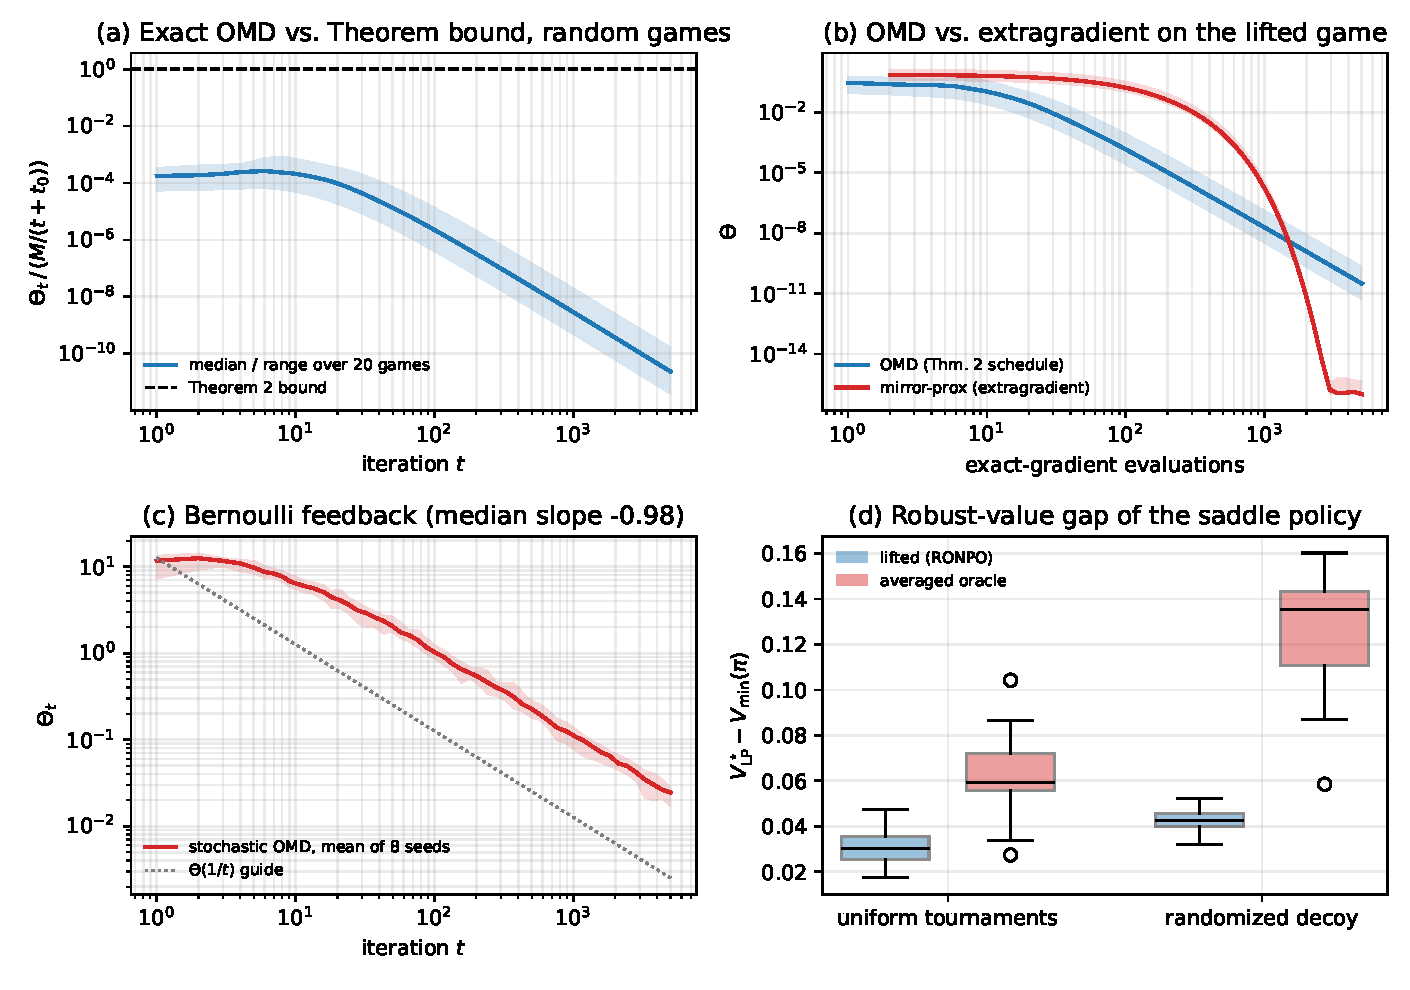
\includegraphics[width=0.95\textwidth]{figures/ronpo_random_families.pdf}
\caption{Validation across random game families (20 games per configuration; bands span the min--max range across games, lines are medians). (a)~Exact-OMD Lyapunov value relative to the Theorem~\ref{thm:lastiter} bound; the bound (dashed) holds in every game. (b)~Exact OMD vs.\ mirror-prox (extragradient) on the lifted game at matched exact-gradient budgets: mirror-prox is linearly convergent, OMD follows $O(1/T)$. (c)~Single-pair Bernoulli feedback, mean of 8 seeds per game (Cor.~\ref{cor:stochastic}). (d)~Robust-value gap $V^\star_{\mathrm{LP}}-V_{\min}(\pi)$ of the saddle policy for the lifted game vs.\ the averaged oracle, on uniform tournaments and randomized decoy games.}
\label{fig:random-families}
\end{figure*}\par}

{\revblue \begin{table}[t]
\centering
\scriptsize
\setlength{\tabcolsep}{3.5pt}
% Numbers generated by toy/random_game_families.py (inlined)
\begin{tabular}{llccc}
\toprule
Axis & Value & Ratio$_{T}$ & Bound & Slope \\
\midrule
base & -- & $2.3\times10^{-11}$ & 20/20 & $-0.98$ \\
$|\mathcal{Y}|$ & 4 & $5.8\times10^{-11}$ & 20/20 & $-1.06$ \\
$|\mathcal{Y}|$ & 16 & $1.8\times10^{-12}$ & 20/20 & $-1.00$ \\
$|\mathcal{Y}|$ & 32 & $5.3\times10^{-14}$ & 20/20 & $-1.00$ \\
$K$ & 2 & $3.0\times10^{-11}$ & 20/20 & $-1.00$ \\
$K$ & 5 & $7.5\times10^{-12}$ & 20/20 & $-1.03$ \\
$K$ & 8 & $7.6\times10^{-12}$ & 20/20 & $-0.97$ \\
coverage & 0.25 & $2.2\times10^{-10}$ & 20/20 & $-1.00$ \\
coverage & 0.5 & $8.0\times10^{-11}$ & 20/20 & $-1.00$ \\
coverage & 0.75 & $3.7\times10^{-11}$ & 20/20 & $-1.08$ \\
$\tau=\kappa$ & 0.01 & $1.1\times10^{-6}$ & 20/20 & $-0.87$ \\
$\tau=\kappa$ & 0.2 & $1.1\times10^{-14}$ & 20/20 & $-1.01$ \\
$\tau=\kappa$ & 0.5 & $1.4\times10^{-14}$ & 20/20 & $-1.02$ \\
noise $\sigma$ & 0.05 & $3.1\times10^{-11}$ & 20/20 & $-1.07$ \\
noise $\sigma$ & 0.1 & $4.5\times10^{-11}$ & 20/20 & $-1.01$ \\
noise $\sigma$ & 0.2 & $1.2\times10^{-10}$ & 20/20 & $-1.03$ \\
\bottomrule
\end{tabular}
\caption{One-at-a-time sensitivity from the base configuration $|\Y|{=}8$, $K{=}3$, coverage $1.0$, $\tau{=}\kappa{=}0.05$, $\sigma{=}0$ (20 random games per row). Ratio$_T$ is the median terminal ratio $\Theta_T/(M/(T+t_0))$ at $T=5000$ for exact OMD; Bound counts games in which the Theorem~\ref{thm:lastiter} bound holds at every recorded iterate; Slope is the median stochastic log--log slope over the final decade (theory: $-1$).}
\label{tab:random-family-sensitivity}
\end{table}\par}

\begin{figure*}[t]
\centering
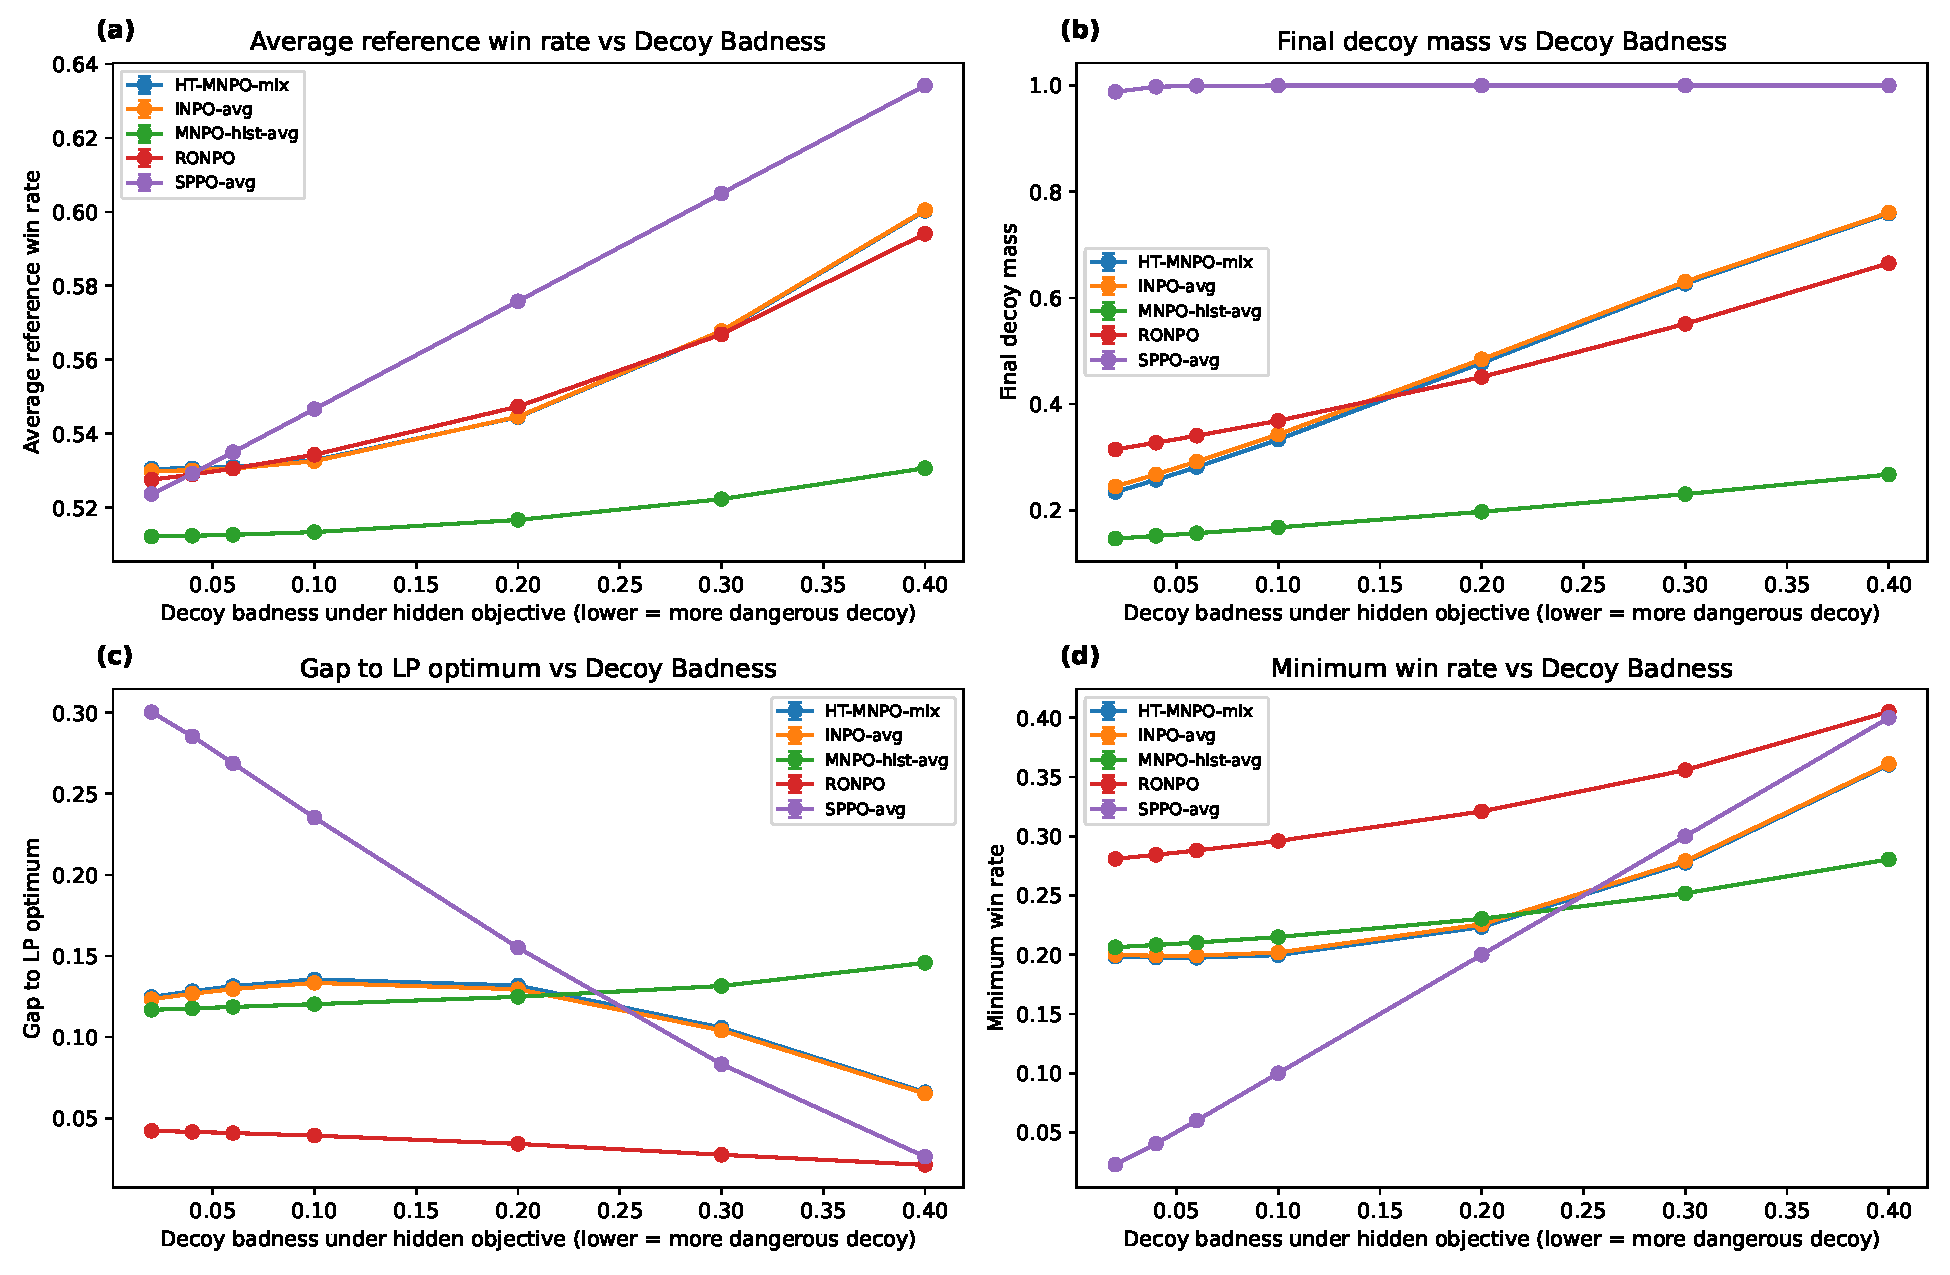
\includegraphics[width=0.95\textwidth]{figures/ronpo_decoy_sweep.pdf}
\caption{Sweep over the hidden-objective decoy win probability $P_3(a_{\mathrm{decoy}}\succ a)$. Lower values make the decoy more dangerous. RONPO is most useful in the regime where the averaged oracle masks severe minority-objective failure.}
\label{fig:decoy-sweep}
\end{figure*}

\begin{figure}[t]
\centering
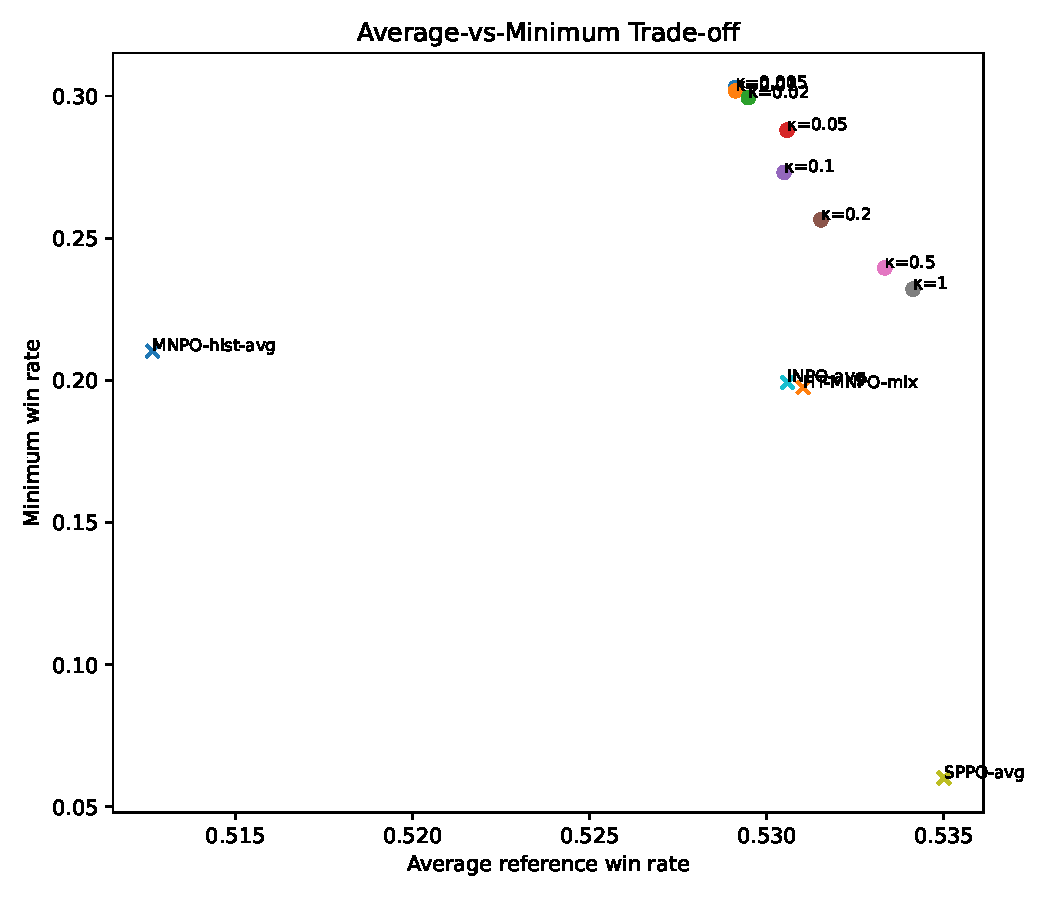
\includegraphics[width=0.98\columnwidth]{figures/kappa_tradeoff_avg_vs_min.pdf}
\caption{RONPO trade-off as the adversary temperature $\kappa$ varies. Smaller $\kappa$ gives a sharper worst-case adversary; larger $\kappa$ moves toward fixed scalarization.}
\label{fig:kappa}
\end{figure}

\section{LLM Experiment Details}
\label{app:llm-details}

\subsection{Stage-1 Evaluation}
\label{app:stage1}

\paragraph{Compared models and training signals.}
All methods are initialized from \texttt{Qwen/Qwen2.5-1.5B-Instruct}. HT-MNPO and RONPO share the same stage-1 base-policy response pool; SPPO-avg and INPO-avg use the prompt-wise average of the min--max-normalized objectives.

{\revblue \paragraph{Training configuration.}
Table~\ref{tab:stage1-common-config} summarizes the common stage-1 configuration for HT-MNPO and RONPO; Table~\ref{tab:stage1-method-config} gives method-specific settings. The SPPO-avg and INPO-avg artifacts record the checkpoint and oracle construction but not the complete optimizer configuration; we do not infer unrecorded hyperparameters. No common hyperparameter search was run across all methods: HT-MNPO and RONPO use the fixed settings above, while SPPO-avg and INPO-avg were retrained under a stability-gated sweep after their original runs failed the generation gate, and the surviving configurations are the ones reported. We state this asymmetry, and the absence of per-method attempt counts for the original artifacts, as a protocol limitation of the 1.5B study.\par}

\begin{table*}[t]
\centering
\footnotesize
\setlength{\tabcolsep}{5pt}
\begin{tabular}{p{0.26\textwidth}p{0.67\textwidth}}
\toprule
Setting & Value \\
\midrule
Base policy & \texttt{Qwen/Qwen2.5-1.5B-Instruct} \\
Training split & UltraFeedback subset; 19{,}856 prompts \\
Held-out split & UltraFeedback subset; 647 prompts \\
Online generation & vLLM with seeds \texttt{13, 21, 42, 79, 100}, temperature 0.8, top-$p$ 0.95, at most 4096 new tokens \\
Objectives & Skywork, Athene, and ArmoRM \\
Shared stage-1 data & HT-MNPO and RONPO use the same base-policy response pool \\
Optimization & bf16 AdamW, learning rate $5\times10^{-7}$, cosine schedule, warmup ratio 0.1, weight decay 0 \\
Training horizon & One epoch; seed 42 \\
Batching & Per-device batch size 2; gradient accumulation 8 \\
Sequence limits & Maximum sequence length 2048; maximum prompt length 1800 \\
Memory and launch & Gradient checkpointing (\texttt{use\_reentrant=false}); Accelerate with DeepSpeed ZeRO-3 \\
\bottomrule
\end{tabular}
\caption{Common stage-1 training configuration for HT-MNPO and RONPO.}
\label{tab:stage1-common-config}
\end{table*}

\begin{table*}[t]
\centering
\footnotesize
\setlength{\tabcolsep}{5pt}
\begin{tabular}{p{0.21\textwidth}p{0.35\textwidth}p{0.35\textwidth}}
\toprule
Setting & HT-MNPO stage 1 & RONPO stage 1 \\
\midrule
Objective handling & One homogeneous oracle per run & Skywork, Athene, and ArmoRM jointly \\
Pair or target construction & Reward-gap target; no target normalization & Per-objective min--max normalization; adversarial pair selection; best-vs-adversary policy pair \\
Method scales & Ratio 0.3333; $\eta=0.0075$; $\beta=(10,1,10)$ for Skywork, Athene, ArmoRM & Policy $\alpha=1.0$; $\tau=0.05$; preference scale $\lambda=8.0$; $\beta=10$ \\
Adversary settings & Not applicable & 25 adversary steps; adversary $\alpha=1.0$; $\kappa=0.05$; one pair per prompt \\
\bottomrule
\end{tabular}
\caption{Method-specific stage-1 training configuration.}
\label{tab:stage1-method-config}
\end{table*}

{\revblue \paragraph{Evaluation configuration and metrics.}
For evaluation, every model generates one response per prompt under identical vLLM decoding (seed 42, temperature 0.7, top-$p$ 0.9, at most 2048 new tokens), and all outputs are rescored by the same three reward models in one pass (Table~\ref{tab:stage1-pairwise}). Let $r_{i,o,m}$ be the score on prompt $i$ from objective $o$ for model $m$. Because reward scales differ, we report per-prompt min--max-normalized scores
\begin{equation}
\widehat r_{i,o,m}
=
\frac{r_{i,o,m}-\min_{m'}r_{i,o,m'}}
{\max_{m'}r_{i,o,m'}-\min_{m'}r_{i,o,m'}},
\label{eq:stage1-normalization}
\end{equation}
with $\widehat r_{i,o,m}=1/2$ when the denominator is zero, averaged over prompts; the extrema range over the exact compared model set, so normalized values are comparable only within one table. Win rates against the base use $w=1$ if $r_{i,o,m}>r_{i,o,m_0}$, $w=0$ if smaller, and $w=1/2$ on exact ties. Aggregates are computed at the objective level: Avg is the mean of the three objective-level means and Worst is their minimum, the worst objective mean of the Experiments section (this differs from the per-prompt worst used on SafeRLHF); the normalized standard deviation is computed across the three objective-level normalized scores.\par}

\begin{table*}[t]
\centering
\scriptsize
\setlength{\tabcolsep}{2.4pt}
\resizebox{\textwidth}{!}{%
\begin{tabular}{lrrrrrrrrrrr}
\toprule
& \multicolumn{2}{c}{Skywork} & \multicolumn{2}{c}{Athene} & \multicolumn{2}{c}{ArmoRM} & \multicolumn{3}{c}{Normalized aggregate} & \multicolumn{2}{c}{WR aggregate} \\
\cmidrule(lr){2-3}\cmidrule(lr){4-5}\cmidrule(lr){6-7}\cmidrule(lr){8-10}\cmidrule(lr){11-12}
Method & Norm. & WR & Norm. & WR & Norm. & WR & Avg. & Worst & Std. & Avg. & Worst \\
\midrule
Base & 0.3990 & -- & 0.4116 & -- & 0.4846 & -- & 0.4317 & 0.3990 & 0.0378 & -- & -- \\
HT-MNPO (Sky.) & 0.4666 & 55.95 & 0.4813 & 58.19 & 0.5529 & 58.73 & 0.5002 & 0.4666 & 0.0377 & 57.62 & 55.95 \\
HT-MNPO (Ath.) & 0.4749 & 56.03 & 0.4225 & 49.69 & 0.4880 & 49.61 & 0.4618 & 0.4225 & 0.0283 & 51.78 & 49.61 \\
HT-MNPO (Armo) & 0.4615 & 56.34 & 0.4356 & 55.72 & 0.4806 & 50.70 & 0.4592 & 0.4356 & \underline{0.0184} & 54.25 & 50.70 \\
RONPO & \textbf{0.6331} & \textbf{67.47} & \underline{0.6432} & \textbf{68.55} & \textbf{0.6339} & \underline{59.81} & \textbf{0.6367} & \textbf{0.6331} & \textbf{0.0046} & \textbf{65.28} & \underline{59.81} \\
SPPO-avg & 0.5131 & 59.51 & 0.4194 & 52.94 & 0.4583 & 48.92 & 0.4636 & 0.4194 & 0.0384 & 53.79 & 48.92 \\
INPO-avg & \underline{0.5962} & \underline{64.30} & \textbf{0.6768} & \underline{67.31} & \underline{0.6208} & \textbf{60.43} & \underline{0.6313} & \underline{0.5962} & 0.0337 & \underline{64.01} & \textbf{60.43} \\
\bottomrule
\end{tabular}%
}
\caption{Stage-1 local reward-model evaluation. \textit{Norm.} is the per-prompt normalized reward and \textit{WR} the win rate against the base response (\%). Lower normalized standard deviation indicates more balanced objective-level performance. RONPO attains the best average and worst-objective normalized reward and the most balanced objective profile; the repaired INPO-avg is the strongest baseline and edges RONPO on the Athene objective.}
\label{tab:stage1-local-rm}
\end{table*}

\begin{table}[t]
\centering
\small
\begin{tabular}{lp{0.6\linewidth}}
\toprule
Objective & Reward model \\
\midrule
Skywork & \path{Skywork/Skywork-Reward-V2-Llama-3.1-8B} \\
Athene & \path{Nexusflow/Athene-RM-8B} \\
ArmoRM & \path{RLHFlow/ArmoRM-Llama3-8B-v0.1} \\
\bottomrule
\end{tabular}
\caption{The three heterogeneous reward models used as the stage-1 objectives.}
\label{tab:stage1-pairwise}
\end{table}

\subsection{Stage-2 Evaluation}
\label{app:stage2}

{\revblue \paragraph{Compared artifacts and setup.}
Stage 2 resumes training from stage-1 checkpoints, comparing the base model, the three single-oracle HT-MNPO checkpoints, and RONPO (an earlier diagnostic RONPO stage-2 run is excluded because it exhibited output-length pathology; the resumed run reported here does not). The exclusion criterion is deterministic, generation-level length pathology detected before any reward evaluation, and the excluded run together with the repaired averaged-oracle baselines of Appendix~\ref{app:stage1} are the only reruns in this study; because retry budgets were not pre-registered uniformly across methods, we flag residual survivorship risk explicitly rather than claiming a fully symmetric selection protocol. The local reward-model and GPT-5.5 evaluations share the same generated responses, so they differ only in the evaluator; IFEval measures rule-based instruction following on a separate benchmark with deterministic decoding.\par}

\kekim{\textbf{[MAJOR]} Excluding a pathological RONPO run while reporting only successful selected checkpoints creates survivorship bias unless the same pre-registered stability gate and retry budget are applied to every method. Report all attempted runs, failure rates, and the deterministic exclusion rule; count failed runs in a stability metric rather than silently replacing them.}

\paragraph{External-judge protocol.}
The judge receives the prompt and two candidate responses labeled A and B, in a deterministically randomized order seeded by the prompt hash, and returns a single preference (A, B, or tie) under a fixed rubric covering helpfulness, correctness, and instruction following. Each unordered pair is judged once per prompt; a tie counts as $0.5$ for both sides. Mean pairwise win rates and $95\%$ intervals use 2000 prompt-level paired bootstrap resamples.

{\revblue \begin{table}[t]
\centering
\small
\setlength{\tabcolsep}{4pt}
\begin{tabular}{lcc}
\toprule
Method & Mean pairwise WR & 95\% CI \\
\midrule
RONPO & \textbf{0.5927} & [0.5709, 0.6136] \\
Base & 0.5581 & [0.5329, 0.5841] \\
HT-MNPO (Sky.) & 0.5054 & [0.4841, 0.5272] \\
HT-MNPO (Armo) & 0.4263 & [0.4025, 0.4493] \\
HT-MNPO (Ath.) & 0.3643 & [0.3425, 0.3855] \\
\bottomrule
\end{tabular}
\caption{Reward-model-independent GPT-5.5 all-pairwise judge results on 647 held-out prompts. Each of the five methods is compared against the other four; the averaged-oracle baselines are not part of this tournament (see Baselines). Higher mean pairwise win rate is better; the per-cell head-to-head matrix accompanies the code release.}
\label{tab:stage2-gpt55}
\end{table}\par}

\kekim{\textbf{[MAJOR]} The table contains five methods, so each can be compared against only four others, not five. More importantly, the promised SPPO-avg and INPO-avg methods are absent. Correct the protocol/count and include the full pairwise matrix so readers can verify the stated head-to-head range.}

\subsection{SafeRLHF Helpfulness--Harmlessness Experiment}
\label{app:saferlhf}
This appendix documents the model-scale SafeRLHF runs summarized in Table~\ref{tab:saferlhf-robust}. Every method starts from \texttt{Llama-3.1-8B-Instruct} and trains for four iterative stages: stage~1 optimizes from the base policy, and stages~2--4 each resume from the previous stage while keeping the base policy as the reference anchor. All methods share the base policy, the training prompts, and the response pools, so the comparison isolates the training signal. Table~\ref{tab:saferlhf-common-config} lists the configuration common to every method and stage, Table~\ref{tab:saferlhf-method-config} the method-specific settings, and Table~\ref{tab:saferlhf-eval-config} the evaluation protocol.

{\revblue \begin{table*}[t]
\centering
\footnotesize
\setlength{\tabcolsep}{5pt}
\begin{tabular}{p{0.26\textwidth}p{0.67\textwidth}}
\toprule
Setting & Value \\
\midrule
Base policy & \path{meta-llama/Llama-3.1-8B-Instruct} \\
Training data & PKU-SafeRLHF \citep{dai2024safe}, train split restricted to the human dual-preference conflicts in which the more helpful response is the less safe one; 2{,}500 prompts per stage \\
Objectives & Helpfulness from the Beaver reward model \path{PKU-Alignment/beaver-7b-v1.0-reward}; harmlessness from the negated Beaver cost model \path{PKU-Alignment/beaver-7b-v1.0-cost} \\
Response pool & vLLM, four responses per prompt; stage~1 from the base policy (seeds 42--45), stages~2--4 mix parent-policy (seeds 42, 43) and base (seeds 44, 45) responses; temperature 0.7, top-$p$ 0.9, at most 512 new tokens, bf16 \\
Pair construction & Three pairs per prompt, selected deterministically; the preferred response has the higher mean of the two per-prompt min--max-normalized objectives; preference scale $\lambda=8.0$ \\
Optimization & bf16 AdamW, learning rate $5\times10^{-7}$, cosine schedule, warmup ratio 0.1, weight decay 0, gradient clipping 1.0 \\
Training horizon & 900 optimizer steps per stage; one independent four-stage run per training seed in $\{42,43,44\}$. The training seed drives data ordering and optimizer stochasticity; decode seeds are unchanged across runs, yet the parent-policy portions of the stage-2--4 pools still differ across training seeds because the parent policies differ. Evaluation decoding and bootstrap seeds stay fixed at 42 \\
Batching & Per-device batch size 1; gradient accumulation 16 \\
Sequence limits & Maximum sequence length 2048; maximum prompt length 1024 \\
Regularizers & Reference-anchor weight 0.05; preference-SFT weight 0.005 \\
Memory and launch & Gradient checkpointing (\texttt{use\_reentrant=false}); single-GPU Accelerate \\
\bottomrule
\end{tabular}
\caption{Common training configuration for the SafeRLHF experiment.}
\label{tab:saferlhf-common-config}
\end{table*}\par}

\kekim{\textbf{[MAJOR]} The configuration table says ``seed 42'' although the results claim training seeds 42, 43, and 44, and the response-pool row specifies stages 1--3 but not stage 4. Resolve both omissions and state which randomness changes across training seeds: initialization, data order, generation pool, or all of them. Reproducible multi-seed claims require independent stochastic training runs, not only different generation seeds.}

\begin{table*}[t]
\centering
\footnotesize
\setlength{\tabcolsep}{5pt}
\begin{tabular}{p{0.24\textwidth}p{0.12\textwidth}p{0.57\textwidth}}
\toprule
Method & Loss & Method-specific settings \\
\midrule
RONPO & \texttt{ronpo} & Objective-stratified target at adversary temperature $\kappa=0.1$; policy $\alpha=1.0$; $\tau=0.05$; closed-form entropic adversary over the two objectives, one opponent sampled per objective \\
HT-MNPO (help./harml.) & \texttt{ht\_mnpo} & One homogeneous oracle per run (helpfulness or harmlessness); reward-gap target; $\eta=0.0075$ \\
INPO-avg & \texttt{inpo} & Prompt-wise average of the normalized objectives; $\eta=0.0075$; ratio 0.3333 \\
SPPO-avg & \texttt{sppo} & Prompt-wise average of the normalized objectives; per-response win-rate target; $\eta=0.0075$ \\
SimPO & \texttt{simpo} & $\beta=2.0$; $\gamma=0.6$ \\
IPO & \texttt{ipo} & $\beta=0.05$; squared log-ratio loss \\
DPO & \texttt{dpo} & $\beta=0.05$; length-normalized \\
\bottomrule
\end{tabular}
\caption{Method-specific training configuration for the SafeRLHF experiment. All methods share the common configuration in Table~\ref{tab:saferlhf-common-config}.}
\label{tab:saferlhf-method-config}
\end{table*}

\begin{table*}[t]
\centering
\footnotesize
\setlength{\tabcolsep}{5pt}
\begin{tabular}{p{0.26\textwidth}p{0.67\textwidth}}
\toprule
Setting & Value \\
\midrule
Evaluation panel & 1{,}000 PKU-SafeRLHF prompts from the official default test split, prompt-disjoint from training and from every intermediate split \\
Generation & vLLM, seed 42, temperature 0.7, top-$p$ 0.9, at most 512 new tokens, bf16 \\
Scoring & Every response rescored by both Beaver heads; helpfulness is the reward and harmlessness is the negated cost \\
Normalization & Per-prompt min--max over the compared policies; Avg and Worst take the mean and minimum across the two objectives \\
Stability gate & Fail-closed per policy: 1{,}000 non-empty responses, no leaked reasoning spans, mean length within $[0.33, 2.0]$ of the base policy, and at most 20 consecutive identical words \\
Confidence intervals & 2{,}000 prompt-level paired bootstrap resamples, seed 42 \\
\bottomrule
\end{tabular}
\caption{Evaluation configuration for the SafeRLHF experiment.}
\label{tab:saferlhf-eval-config}
\end{table*}

{\revblue \subsection{Qwen3-8B Instruction-Following Scale-Up}
\label{app:qwen3-ifeval}
This diagnostic tests whether the instruction-following preservation seen at 1.5B survives a larger policy, training on \texttt{Qwen3-8B} under three heterogeneous ArmoRM objectives (helpfulness, safety, and conciseness; Appendix~\ref{app:qwen3-robust}). Table~\ref{tab:qwen3-ifeval} reports the four official IFEval aggregations. Because the reported configurations were selected on this same benchmark, the table is validation evidence, not test evidence, and the between-method differences are small; we therefore draw no comparative conclusion from it and use it only as a sanity check that preference optimization at this scale does not damage instruction following. A clean protocol, selecting configurations on a separate validation split and running the official test once, is deferred to the revision. This study also uses a different base model from the SafeRLHF experiment of Appendix~\ref{app:saferlhf}, so the IFEval numbers here and the reward-based results there do not describe a single 8B policy.\par}

{\revblue \begin{table}[t]
\centering
\scriptsize
\setlength{\tabcolsep}{4pt}
\begin{tabular}{lrrrr}
\toprule
& \multicolumn{2}{c}{Strict} & \multicolumn{2}{c}{Loose} \\
\cmidrule(lr){2-3}\cmidrule(lr){4-5}
Method & Prompt & Inst. & Prompt & Inst. \\
\midrule
Base  & 0.8336 & 0.8900 & 0.8651 & 0.9140 \\
DPO   & 0.8281 & 0.8808 & 0.8688 & 0.9122 \\
SPPO  & 0.8281 & 0.8811 & 0.8614 & 0.9036 \\
SimPO & \textbf{0.8466} & \underline{0.8943} & \underline{0.8799} & \underline{0.9187} \\
RONPO & \underline{0.8410} & \textbf{0.8962} & \textbf{0.8817} & \textbf{0.9276} \\
\bottomrule
\end{tabular}
\caption{Qwen3-8B scale-up diagnostic on all IFEval prompts, reporting all four official aggregations. Rows are configurations selected on this same benchmark from fixed method sweeps, so the table is a sanity check of instruction-following preservation, not an untouched-test comparison.}
\label{tab:qwen3-ifeval}
\end{table}\par}

{\revblue \subsection{Qwen3-8B Heterogeneous-Objective Diagnostic}
\label{app:qwen3-robust}
As a second model-scale probe, we ran a Qwen3-8B diagnostic on a sealed held-out test with three conflicting ArmoRM objectives (helpfulness, safety, conciseness). The study is underpowered: across the ten stable policies the mean raw rewards span at most $\QwenArmoMaxSpread$ per objective, so per-prompt normalization amplifies statistically indistinguishable differences and the resulting ordering diagnoses evaluator power, not model robustness; pre-committed rescoring with two general reward models likewise separates no trained policy from base. We record this as honest negative evidence, defer the full diagnostic to the supplementary material, and will precede any future scale-up with an a priori evaluator power analysis.\par}

{\revblue \subsection{Qwen3-8B Capability Preservation}
\label{app:qwen3-academic}
We check that preference optimization at the 8B backbone does not damage general capability, using a shared seed-42 academic suite under lm-evaluation-harness 0.4.12 with thinking disabled and fixed per-task shot counts. Table~\ref{tab:qwen3-academic} reports the accessible benchmarks with a macro average and its signed difference from the base policy. The macro is the mean of the six benchmarks shown. GPQA is omitted because the official dataset is access-gated, and HumanEval is excluded from the macro entirely: a think-mode chat-template failure prevents the harness from extracting code for every model, and a broken task does not belong in a capability aggregate even as a constant offset; we will rerun it once the extraction is fixed. All runs use a single seed and most per-task deltas are within run-to-run noise, so we read the table as showing no evidence of capability damage rather than as a ranking among methods.\par}

{\revblue % Numbers auto-generated by analysis/ronpo_8b_reconstruction_20260714/build_ronpo_8b_tables_figure.py
% Macro recomputed by hand over the six displayed tasks (HumanEval excluded); update the builder accordingly when regenerating.
\begin{table}[t]
\centering
\scriptsize
\setlength{\tabcolsep}{3pt}
\resizebox{\columnwidth}{!}{%
\begin{tabular}{lrrrrrrr}
\toprule
Method & IFEval & MMLU & MMLU-Pro & ARC & GSM8K & AIME & Macro$_{\Delta}$ \\
\midrule
Base & 80.96 & 72.03 & 63.16 & 63.74 & 81.65 & 26.67 & 64.70$\;(\pm0)$ \\
\midrule
RONPO (top-mass) & 82.44 & 71.99 & 63.07 & 63.65 & 80.97 & 30.00 & 65.35$\,(+0.65)$ \\
RONPO (full-exp.) & 81.52 & 71.97 & 63.00 & 63.57 & 80.89 & 23.33 & 64.05$\,(-0.66)$ \\
DPO & 81.33 & 71.87 & 63.51 & 63.48 & 81.20 & 30.00 & 65.23$\,(+0.53)$ \\
IPO & 82.44 & 71.88 & 63.20 & 63.57 & 81.12 & 33.33 & 65.92$\,(+1.22)$ \\
SimPO & 80.41 & 71.92 & 63.07 & 63.57 & 81.05 & 23.33 & 63.89$\,(-0.81)$ \\
SPPO (avg) & 81.15 & 71.74 & 63.41 & 63.74 & 80.29 & 30.00 & 65.05$\,(+0.35)$ \\
INPO (avg) & 81.52 & 71.83 & 63.31 & 63.65 & 80.52 & 23.33 & 64.03$\,(-0.68)$ \\
HT-MNPO (help.) & 81.15 & 72.08 & 63.39 & 63.65 & 80.52 & 23.33 & 64.02$\,(-0.68)$ \\
HT-MNPO (safety) & 81.89 & 71.89 & 63.37 & 63.65 & 80.89 & 33.33 & 65.84$\,(+1.13)$ \\
HT-MNPO (concise) & 81.89 & 71.71 & 63.57 & 63.23 & 80.59 & 23.33 & 64.05$\,(-0.65)$ \\
\bottomrule
\end{tabular}%
}
\caption{\textbf{Capability preservation} on the shared seed-42 academic suite (lm-evaluation-harness 0.4.12, think disabled). Macro$_{\Delta}$ is the mean over the six displayed benchmarks with the signed difference from base in parentheses; GPQA is access-gated, and HumanEval is excluded because a think-mode code-extraction failure invalidates it for every model. Single seed; per-benchmark deltas are within run-to-run noise (AIME-24 has 30 items, so $\pm3.3$pp equals one problem), so the table supports a no-evidence-of-regression reading rather than a ranking.}
\label{tab:qwen3-academic}
\end{table}\par}

\kekim{\textbf{[MAJOR]} Configuration selection on IFEval makes this table validation evidence, not test evidence, and the differences are very small. Select hyperparameters on a separate validation split, freeze them, and rerun the official test once. Otherwise remove comparative ``best'' language and use this only as a sanity check.}

\kekim{\textbf{[MINOR]} This is honest negative evidence, but the many auto-generated unused macros and detailed diagnostic distract from the central story. Move the full failed diagnostic to supplementary material and summarize it in two sentences. For the revision, perform an a priori power analysis and choose evaluators/tasks with enough dynamic range before launching the expensive scale-up.}

\kekim{\textbf{[MAJOR]} A broken HumanEval pipeline must not be included in a capability macro, even if it adds the same offset to every row; it changes the reported magnitude and signals an unvalidated harness. Fix the chat-template extraction and rerun, or exclude HumanEval from both numerator and denominator. Add task-level uncertainty and avoid ``no regression'' claims from one seed when most deltas are within run-to-run noise.}

\end{document}